%%%%%%%%%%%%%%%%%%%%%%%%%%%%%%%%%%%%%%%%%%%%%%%%%%%%%%%%%%%%%%%%%%%%%%%%%%%%%%%%%%%%%%%%%%%%%%%%%%%%%%%%%%%%%%%
\chapter{$K$ versus $k$}
%%%%%%%%%%%%%%%%%%%%%%%%%%%%%%%%%%%%%%%%%%%%%%%%%%%%%%%%%%%%%%%%%%%%%%%%%%%%%%%%%%%%%%%%%%%%%%%%%%%%%%%%%%%%%%%
!!!!!!!!!!!!!!!!!!!!!!!Skriv en introduksjon og en forklaring på hva $K$ og $k$ er!!!!!!!!!!!!!!!\\
\begin{figure}[H]
        \centering
        \begin{subfigure}[b]{0.3\textwidth}
                \includegraphics[width=\textwidth]{../MATLAB/fig/Kversusktime.jpg}
                \caption{  }
                \label{fig:restarttimeprob1}
        \end{subfigure}
        ~
        \begin{subfigure}[b]{0.3\textwidth}
                \includegraphics[width=\textwidth]{../MATLAB/fig/Kversuskerror.jpg}
                \caption{  }
                \label{fig:restarttimeprob2}
        \end{subfigure}
        ~
        \begin{subfigure}[b]{0.3\textwidth}
                \includegraphics[width=\textwidth]{../MATLAB/fig/Kversuskenergy.jpg}
                \caption{  }
                \label{fig:restarttimeprob2}
        \end{subfigure}
        \caption{ !!!!!!!!!!!!!!!!!SKRIV NOE HER!!!!!!!!!!!!!!!!!!  }
        \label{fig:restarttimeprob}
\end{figure}
!!!!!!!!!!!!!!kommentere resultatene!!!!!!!!!!!!!!!!!!\\

%%%%%%%%%%%%%%%%%%%%%%%%%%%%%%%%%%%%%%%%%%%%%%%%%%%%%%%%%%%%%%%%%%%%%%%%%%%%%%%%%%%%%%%%%%%%%%%%%%%%%%%%%%%%%%%
\chapter{The perfect restart variable}
%%%%%%%%%%%%%%%%%%%%%%%%%%%%%%%%%%%%%%%%%%%%%%%%%%%%%%%%%%%%%%%%%%%%%%%%%%%%%%%%%%%%%%%%%%%%%%%%%%%%%%%%%%%%%%%
!!!!!!!!!!!!!!!!!!!!!!!!!!!!!Skriv en introduksjon om hva restartvariabel er!!!!!!!!!!!!!\\
\begin{figure}[H]
        \centering
        \begin{subfigure}[b]{0.45\textwidth}
                \includegraphics[width=\textwidth]{../MATLAB/fig/restarttime.jpg}
                \caption{  }
                \label{fig:restarttimeprob1}
        \end{subfigure}
        ~
        \begin{subfigure}[b]{0.45\textwidth}
                \includegraphics[width=\textwidth]{../MATLAB/fig/restartiter.jpg}
                \caption{  }
                \label{fig:restarttimeprob2}
        \end{subfigure}
        \begin{subfigure}[b]{0.45\textwidth}
                \includegraphics[width=\textwidth]{../MATLAB/fig/restarterror.jpg}
                \caption{  }
                \label{fig:restarttimeprob2}
        \end{subfigure}
        \begin{subfigure}[b]{0.45\textwidth}
                \includegraphics[width=\textwidth]{../MATLAB/fig/restartenergy.jpg}
                \caption{  }
                \label{fig:restarttimeprob2}
        \end{subfigure}
        \caption{ !!!!!!!!!!!!!!!!!SKRIV NOE HER!!!!!!!!!!!!!!!!!!  }
        \label{fig:restarttimeprob}
\end{figure}
!!!!!!!!!!!!!!!Skriv noen commentarer her!!!!!!!!!!!!!!!!!!!!!!\\


%%%%%%%%%%%%%%%%%%%%%%%%%%%%%%%%%%%%%%%%%%%%%%%%%%%%%%%%%%%%%%%%%%%%%%%%%%%%%%%%%%%%%%%%%%%%%%%%%%%%%%%%%%%%%%%
\chapter{Integrating over looong time}
%%%%%%%%%%%%%%%%%%%%%%%%%%%%%%%%%%%%%%%%%%%%%%%%%%%%%%%%%%%%%%%%%%%%%%%%%%%%%%%%%%%%%%%%%%%%%%%%%%%%%%%%%%%%%%%
!!!!!!!!!!!!!!!!!!!!!!!!!!!!!Skriv en introduksjon om hva restartvariabel er!!!!!!!!!!!!!\\
\begin{figure}[H]
        \centering
        \begin{subfigure}[b]{0.3\textwidth}
                \includegraphics[width=\textwidth]{../MATLAB/fig/longtime10.jpg}
                \caption{  }
                \label{fig:restarttimeprob1}
        \end{subfigure}
        ~
        \begin{subfigure}[b]{0.3\textwidth}
                \includegraphics[width=\textwidth]{../MATLAB/fig/longtime20.jpg}
                \caption{  }
                \label{fig:restarttimeprob2}
        \end{subfigure}
        ~
        \begin{subfigure}[b]{0.3\textwidth}
                \includegraphics[width=\textwidth]{../MATLAB/fig/longtime30.jpg}
                \caption{  }
                \label{fig:restarttimeprob2}
        \end{subfigure}
        
        \begin{subfigure}[b]{0.3\textwidth}
                \includegraphics[width=\textwidth]{../MATLAB/fig/longtime11.jpg}
                \caption{  }
                \label{fig:restarttimeprob2}
        \end{subfigure}
        ~
        \begin{subfigure}[b]{0.3\textwidth}
                \includegraphics[width=\textwidth]{../MATLAB/fig/longtime21.jpg}
                \caption{  }
                \label{fig:restarttimeprob2}
        \end{subfigure}
        ~
        \begin{subfigure}[b]{0.3\textwidth}
                \includegraphics[width=\textwidth]{../MATLAB/fig/longtime31.jpg}
                \caption{  }
                \label{fig:restarttimeprob2}
        \end{subfigure}
        \caption{ !!!!!!!!!!!!!!!!!SKRIV NOE HER!!!!!!!!!!!!!!!!!!  }
        \label{fig:restarttimeprob}
\end{figure}
!!!!!!!!!!!!!!!Skriv noen commentarer her!!!!!!!!!!!!!!!!!!!!!!\\
%%%%%%%%%%%%%%%%%%%%%%%%%%%%%%%%%%%%%%%%%%%%%%%%%%%%%%%%%%%%%%%%%%%%%%%%%%%%%%%%%%%%%%%%%%%%%%%%%%%%%%%%%%%%%%%
\chapter{Some interesting results}
%%%%%%%%%%%%%%%%%%%%%%%%%%%%%%%%%%%%%%%%%%%%%%%%%%%%%%%%%%%%%%%%%%%%%%%%%%%%%%%%%%%%%%%%%%%%%%%%%%%%%%%%%%%%%%%
The energy has already been considered quite thoroughly, but there are still interesting factors to consider. This chapter will show how the different methods compare in relation to computation time, number of iterations, and error. This will be done with  \texttt{wave} and \texttt{semirandom} both with constant and varying energy.\\

!!!!!!!!!!!!!!!!!!!Mange av bildene som er her burde ikke vært her!!!!!!!!!!!!!!!!!\\
!!!!!!!!!!!!!!!!!!!Det mangler myye beskrivelse av bildene!!!!!!!!!!!!!!!!!!!\\
!!!!!!!!!!!!!!!!!!!Finn ut hvilke(om noen) restartvariabler som gir kjappest resultat!!!!!!!!!!!!!\\
!!!!!!!!!!!!!!!!!!!Noen figurer burde ikke være loglog!!!!!!!!!!!!!!!!!!!!!!!!!\\
!!!!!!!!!!!!!!!!!!!Computationtime bildene burde vært bedre!!!!!!!!!!!!!!!!!!!!!!!!!!\\
!!!!!!!!!!!!!!!!!!!Trenger et bedre mål for feilen med semirandom!!!!!!!!!!!!!!!!!!!!!!\\
!!!!!!!!!!!!!!!!!!!Dele opp kapitlene mer fornuftig?!!!!!!!!!!!!!!!!!!!!!!!!!!!!!\\
!!!!!!!!!!!!!!!!!!!Skrive konklusjon og fylle inn steder der det trengs!!!!!!!!!!!!!!\\
!!!!!!!!!!!!!!!!!!!!!!Burde bruke trapes og midpoint rule mange forskjellige steder!!!!!!!!!!!!!!!!!!!\\

\section{The best restartvariable}
%%%%%%%%%%%%%%%%%%%%%%%%%%%%%%%%%%%%%%%%%%%%%%%%%%%%%%%%%%%%%%%%%%%%%%%%%%%%%%%%%%%%%%%%%%%%%%%%%%%%%%%%%%%%%%%
!!!!!!!!!!Finn på en bedre tittel!!!!!!!!!!!!!!!!!!!\\
!!!!!!!!!!!!!!!!!Flere figurer med forskjellige $m$ er!!!!!!!!!!!!!!!!!!\\
\begin{figure}[H]
        \centering
        \begin{subfigure}[b]{0.45\textwidth}
                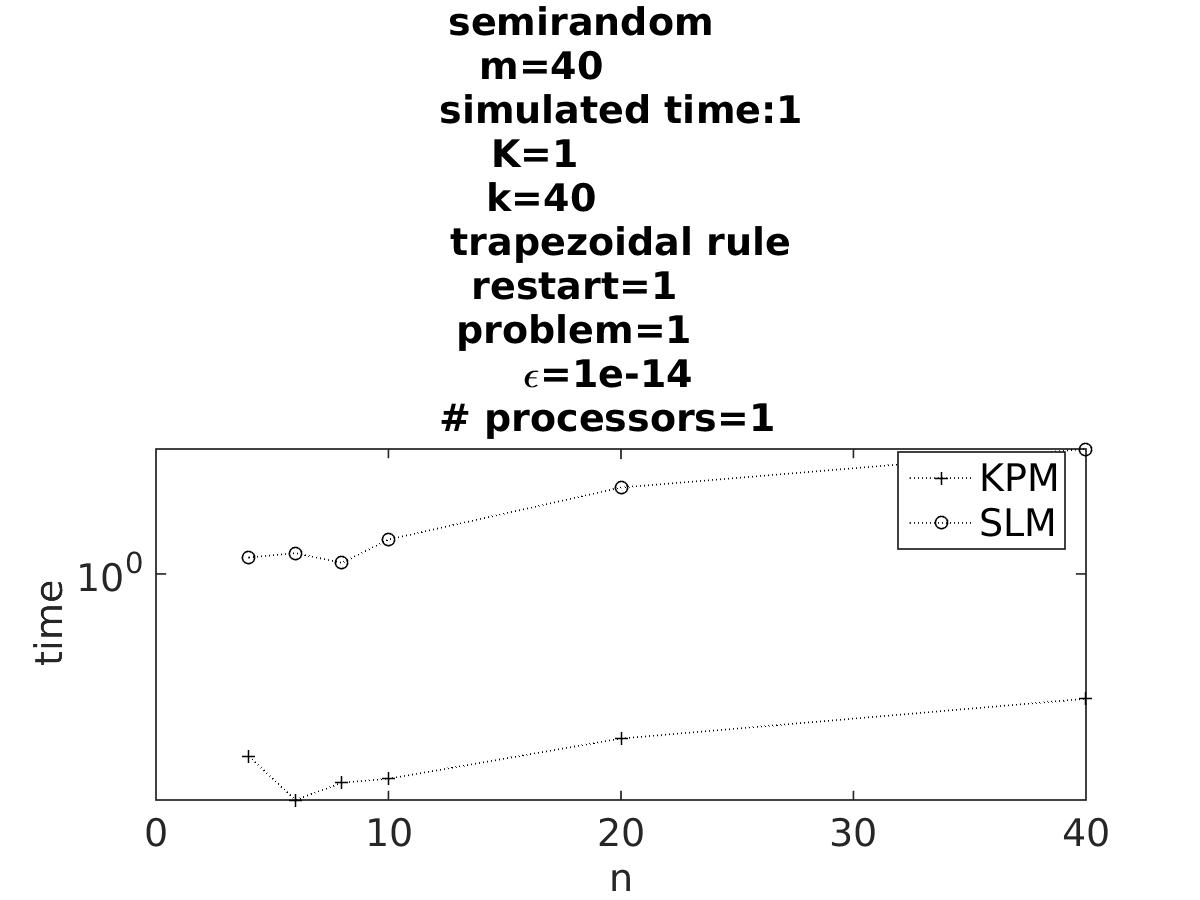
\includegraphics[width=\textwidth]{../MATLAB/fig/restarttimeprob1.jpg}
                \caption{  }
                \label{fig:restarttimeprob1}
        \end{subfigure}
        ~
        \begin{subfigure}[b]{0.45\textwidth}
                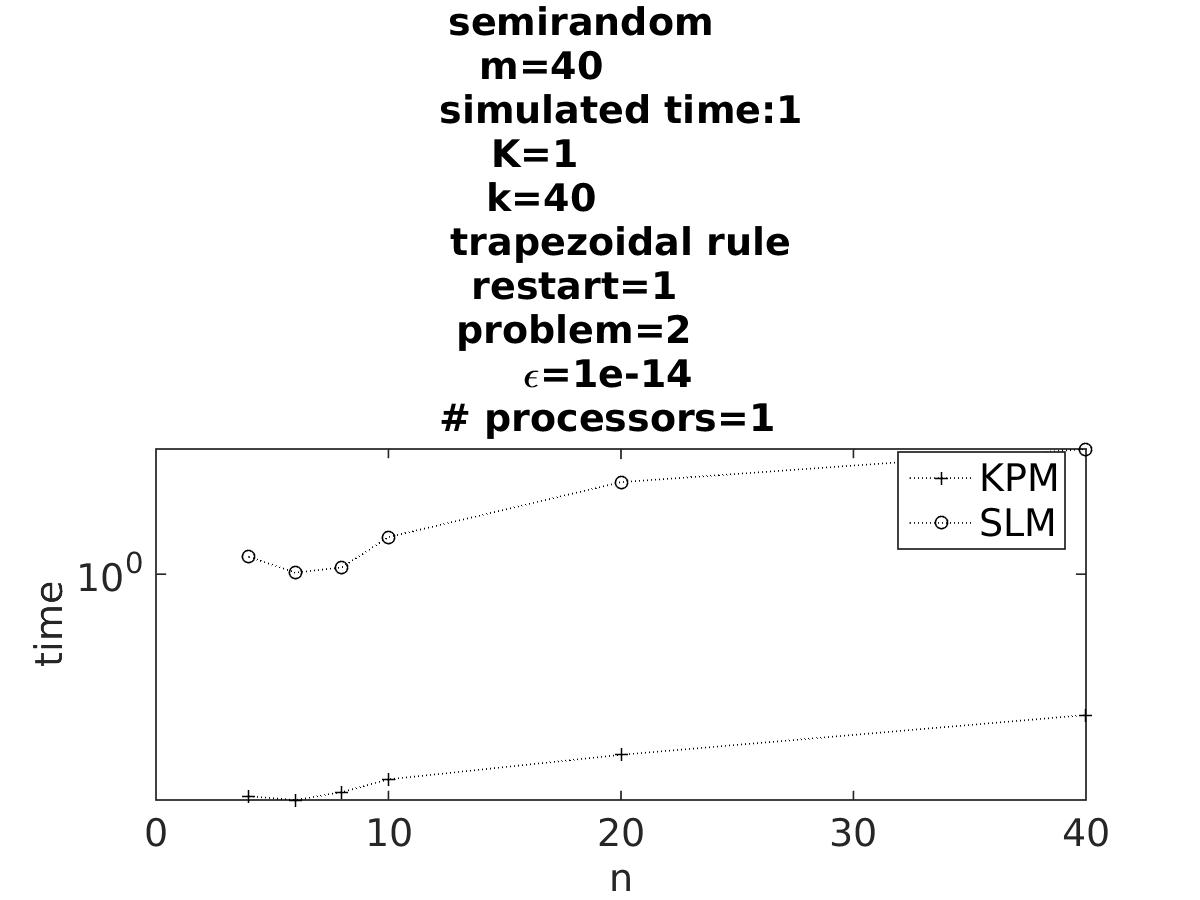
\includegraphics[width=\textwidth]{../MATLAB/fig/restarttimeprob2.jpg}
                \caption{  }
                \label{fig:restarttimeprob2}
        \end{subfigure}
        \caption{ !!!!!!!!!!!!!!!!!SKRIV NOE HER!!!!!!!!!!!!!!!!!!  }
        \label{fig:restarttimeprob}
\end{figure}


\begin{figure}[H]
        \centering
        \begin{subfigure}[b]{0.45\textwidth}
                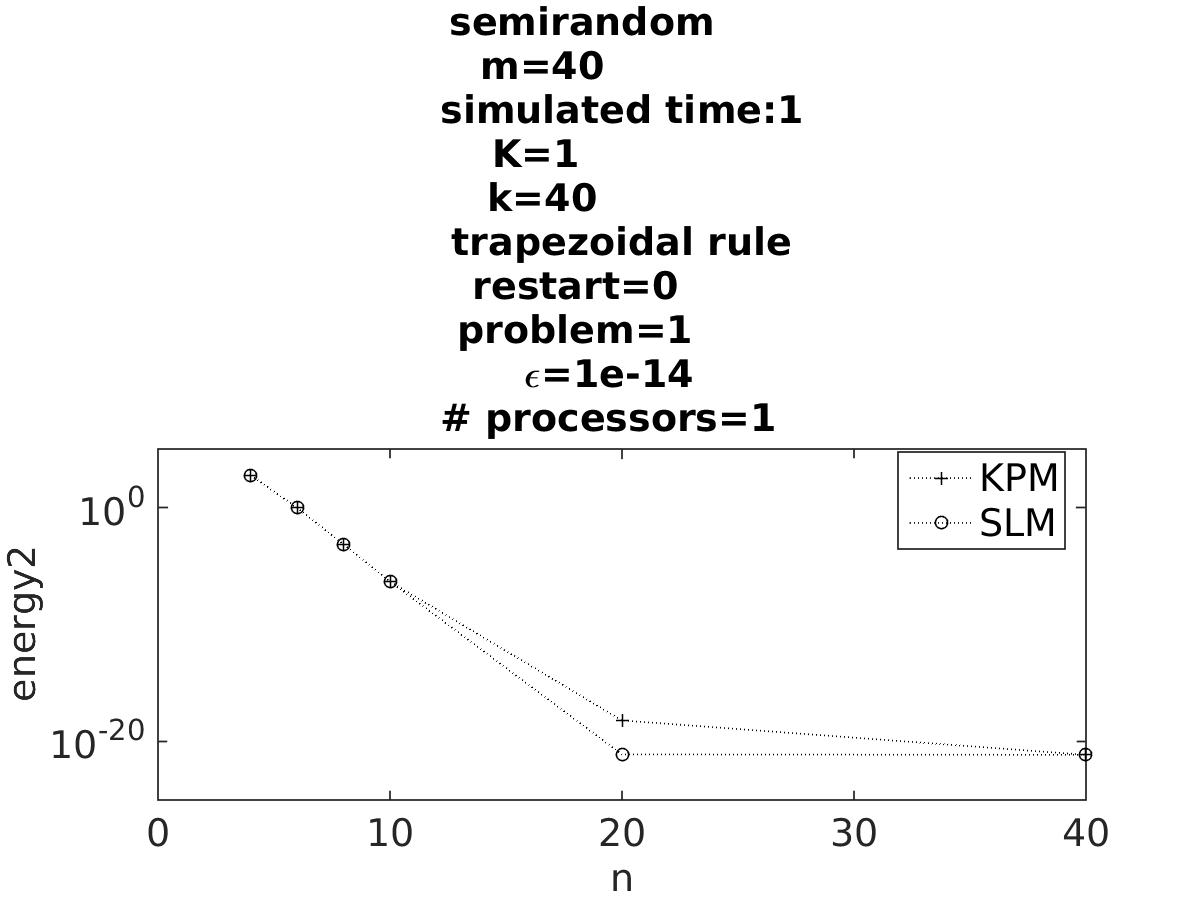
\includegraphics[width=\textwidth]{../MATLAB/fig/restartenergyprob1.jpg}
                \caption{  }
                \label{fig:restarttimeprob1}
        \end{subfigure}
        ~
        \begin{subfigure}[b]{0.45\textwidth}
                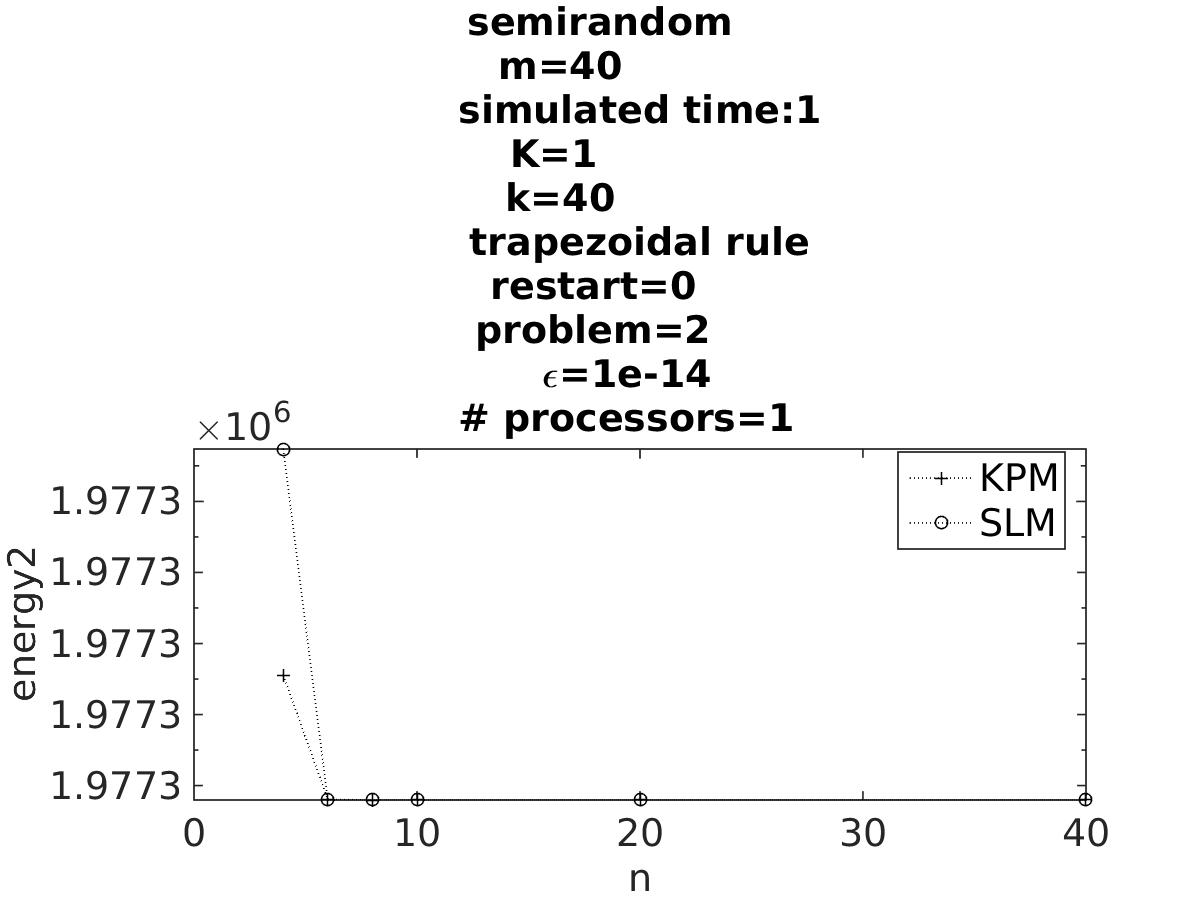
\includegraphics[width=\textwidth]{../MATLAB/fig/restartenergyprob2.jpg}
                \caption{  }
                \label{fig:restarttimeprob2}
        \end{subfigure}
        \caption{ !!!!!!!!!!!!!!!!!SKRIV NOE HER!!!!!!!!!!!!!!!!!!  }
        \label{fig:restarttimeprob}
\end{figure}
!!!!!!!!!!!!!!!!!!!Tekst mangler i dette avsnittet!!!!!!!!!!!!!!!!!!!!!!!!!!!!!!!!!!!!!!!!\\
\section{de greiene med forskjellige K og k!}
%%%%%%%%%%%%%%%%%%%%%%%%%%%%%%%%%%%%%%%%%%%%%%%%%%%%%%%%%%%%%%%%%%%%%%%%%%%%%%%%%%%%%%%%%%%%%%%%%%%%%%%%%%%%%%%
!!!!!!!!!!!!!!!!!!!!!!!Fyll inn noe her!!!!!!!!!!!!!!!!!!!!!!!!!!!!\\
!!!!!!!!!!!!!!!!!!!!!Bilder av error med stor $k$ , og liten $K$, sammenlignet med det motsatte, uten restart!!!!!!!!!!!!!!!!!!!\\
!!!!!!!!!!!!!!!!!!!!!Bilder av error med stor $k$ , og liten $K$, sammenlignet med det motsatte, med restart!!!!!!!!!!!!!!!!!!!\\
!!!!!!!!!!!!!!!!!!!!!!Og med de forskjellige metodene!!!!!!!!!!!!!!!!!!!!!!!!!!!!\\
 

\section{Constant energy with the wave equation}
%%%%%%%%%%%%%%%%%%%%%%%%%%%%%%%%%%%%%%%%%%%%%%%%%%%%%%%%%%%%%%%%%%%%%%%%%%%%%%%%%%%%%%%%%%%%%%%%%%%%%%%%%%%%%%%
% The \texttt{wave} framework will be used due to the need for comparing the difficulty of solving the problem with different sizes.\\
%!!!!!!!!!!!!!!!!!!!!!Dette må gjøres for andre problemer, dette er jo bare teit!!!!!!!!!!!!!!!!!!!!!!!\\
This section will show how the the methods differs with constant energy and the wave equation.



\begin{figure}[H]
        \centering
        \begin{subfigure}[b]{0.45\textwidth}
                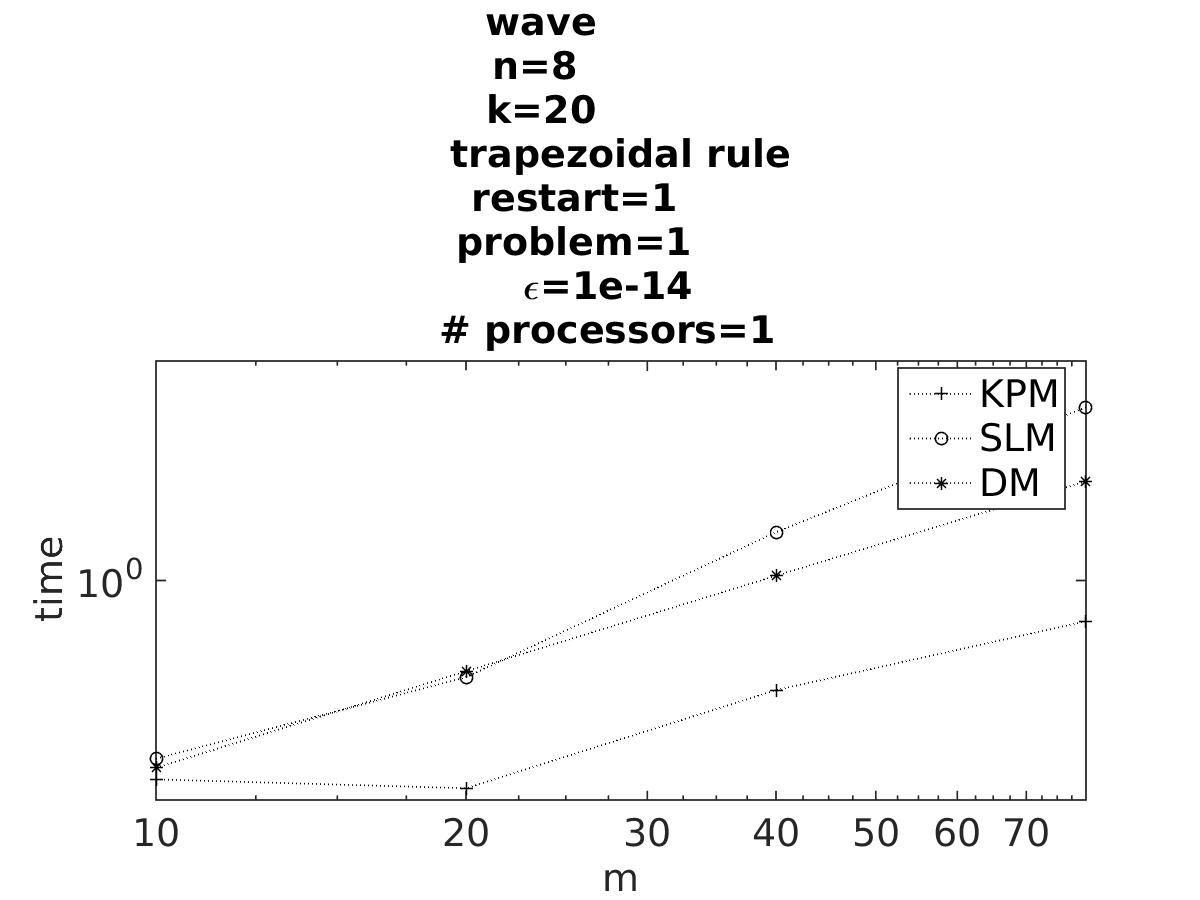
\includegraphics[width=\textwidth]{../MATLAB/fig/resulttimem.jpg}
                \caption{  }
                \label{fig:resulttimem}
        \end{subfigure}
        ~
        \begin{subfigure}[b]{0.45\textwidth}
                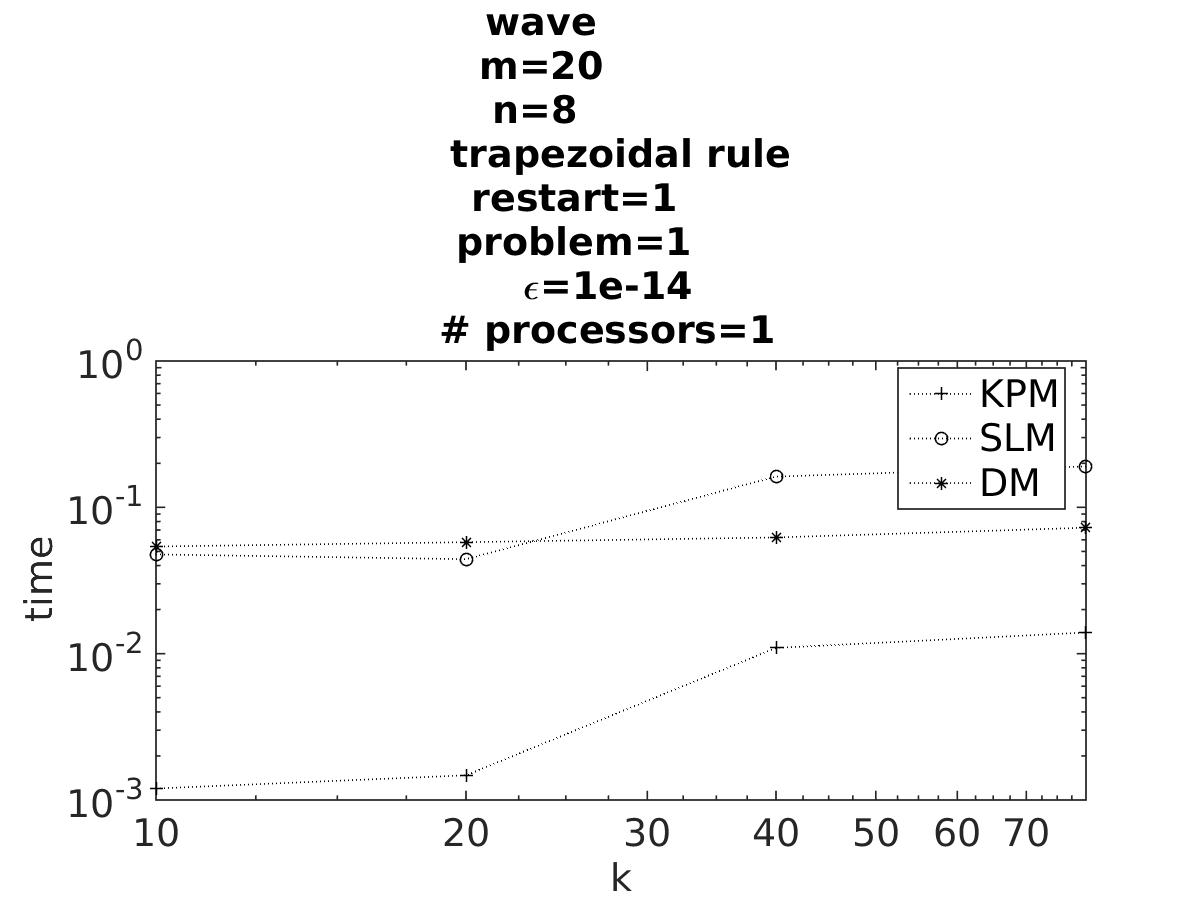
\includegraphics[width=\textwidth]{../MATLAB/fig/resulttimek.jpg}
                \caption{  }
                \label{fig:resulttimek}
        \end{subfigure}
        \caption{ For both cases KPM is faster than the other, and with DM faster than SLM.  }
        \label{fig:resulttime}
\end{figure}



\begin{figure}[H]
        \centering

                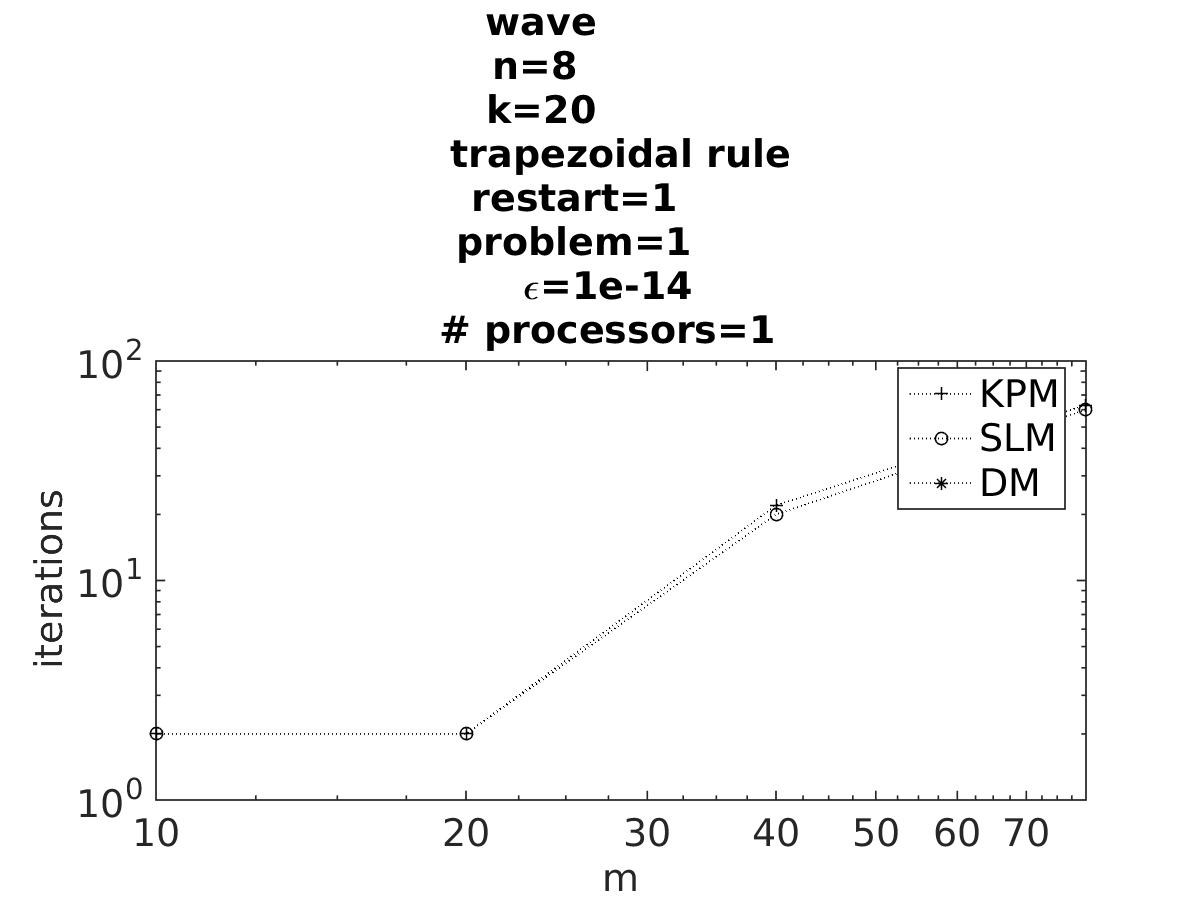
\includegraphics[width=0.45\textwidth]{../MATLAB/fig/resultiter.jpg}
        \label{fig:resultiter}
        \caption{The number of iterations are almost equal for the two methods.}
\end{figure}

\begin{figure}[H]
        \centering
        \begin{subfigure}[b]{0.45\textwidth}
                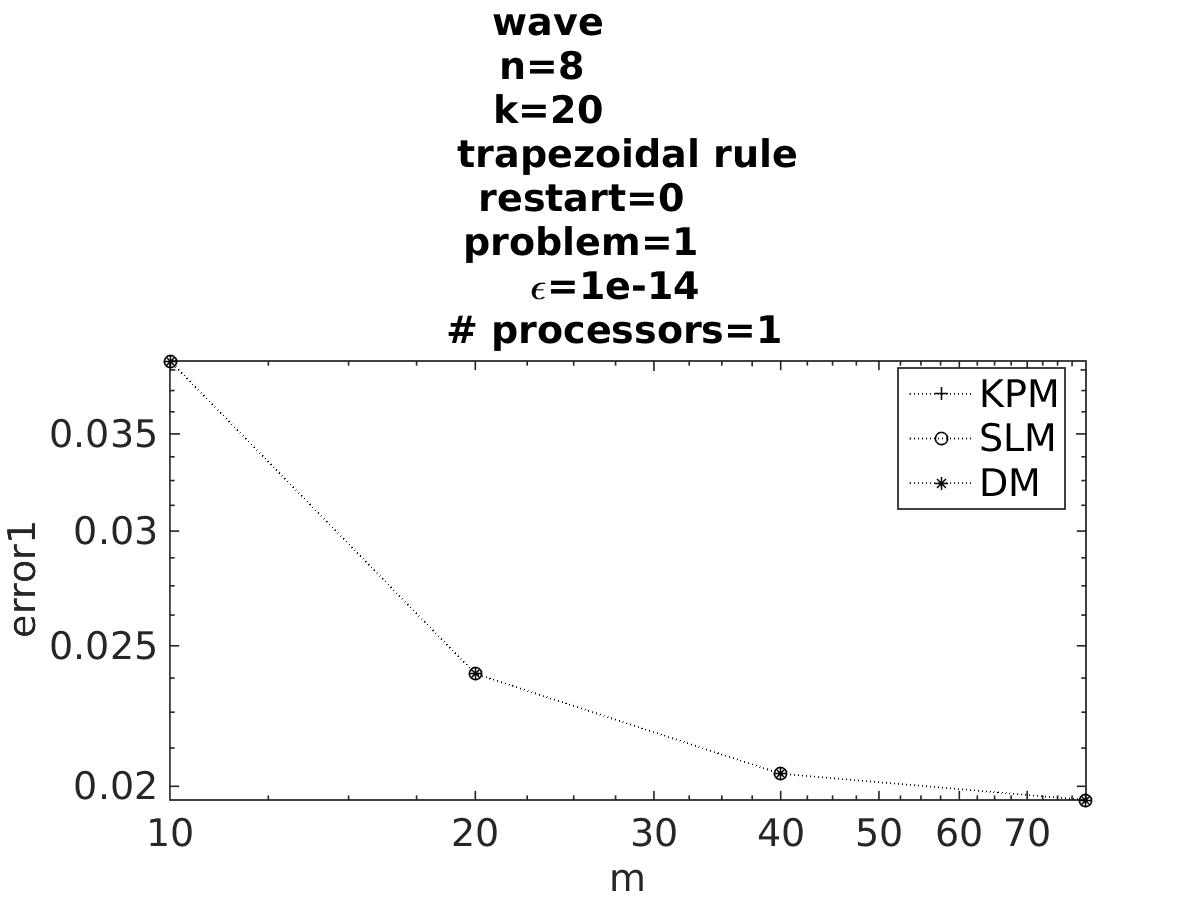
\includegraphics[width=\textwidth]{../MATLAB/fig/resulterrorr.jpg}
                \caption{  }
                \label{fig:resulterror1}
        \end{subfigure}
        ~
        \begin{subfigure}[b]{0.45\textwidth}
                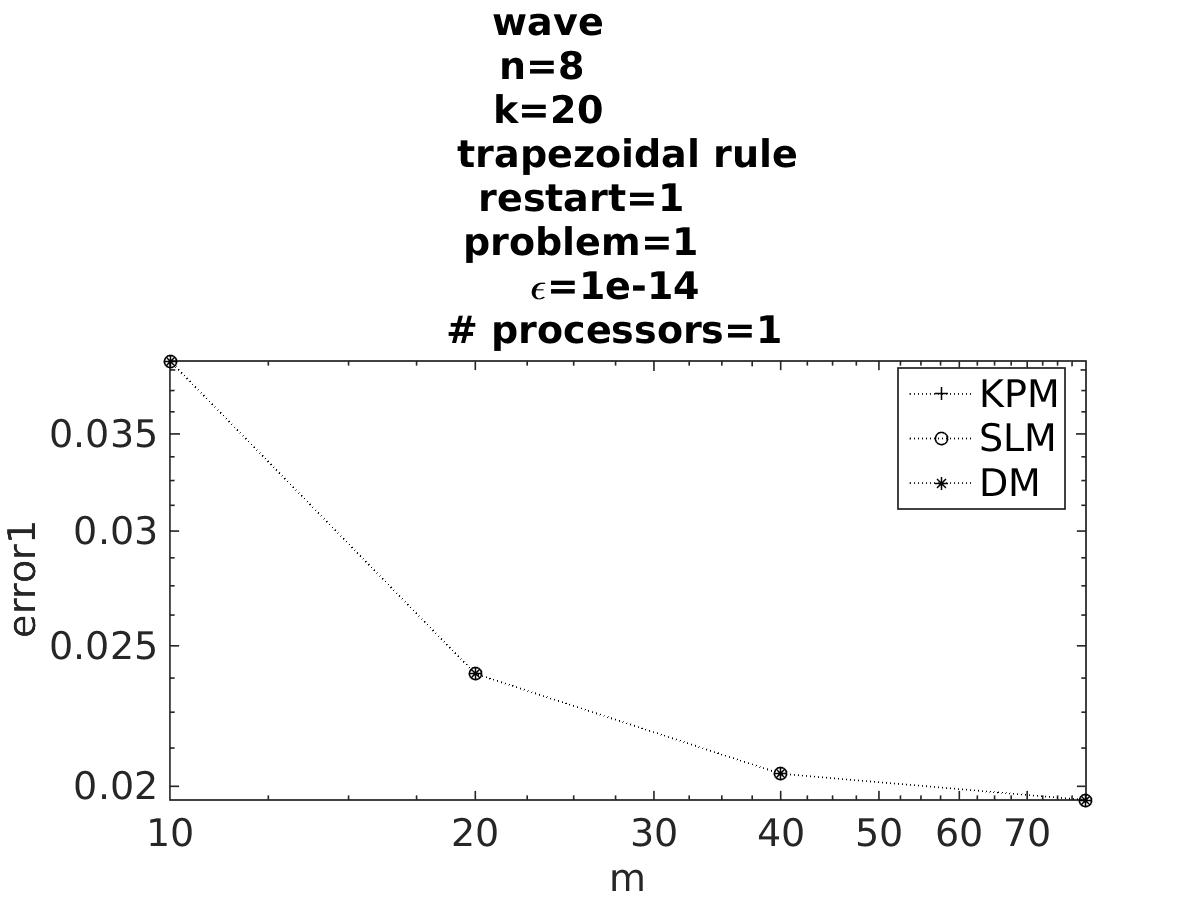
\includegraphics[width=\textwidth]{../MATLAB/fig/resulterror.jpg}
                \caption{  }
                \label{fig:resulterror2}
        \end{subfigure}
        \caption{ The error is nearly identical.  }
        \label{fig:resulterror}
\end{figure}


\begin{figure}[H]
        \centering
        \begin{subfigure}[b]{0.45\textwidth}
                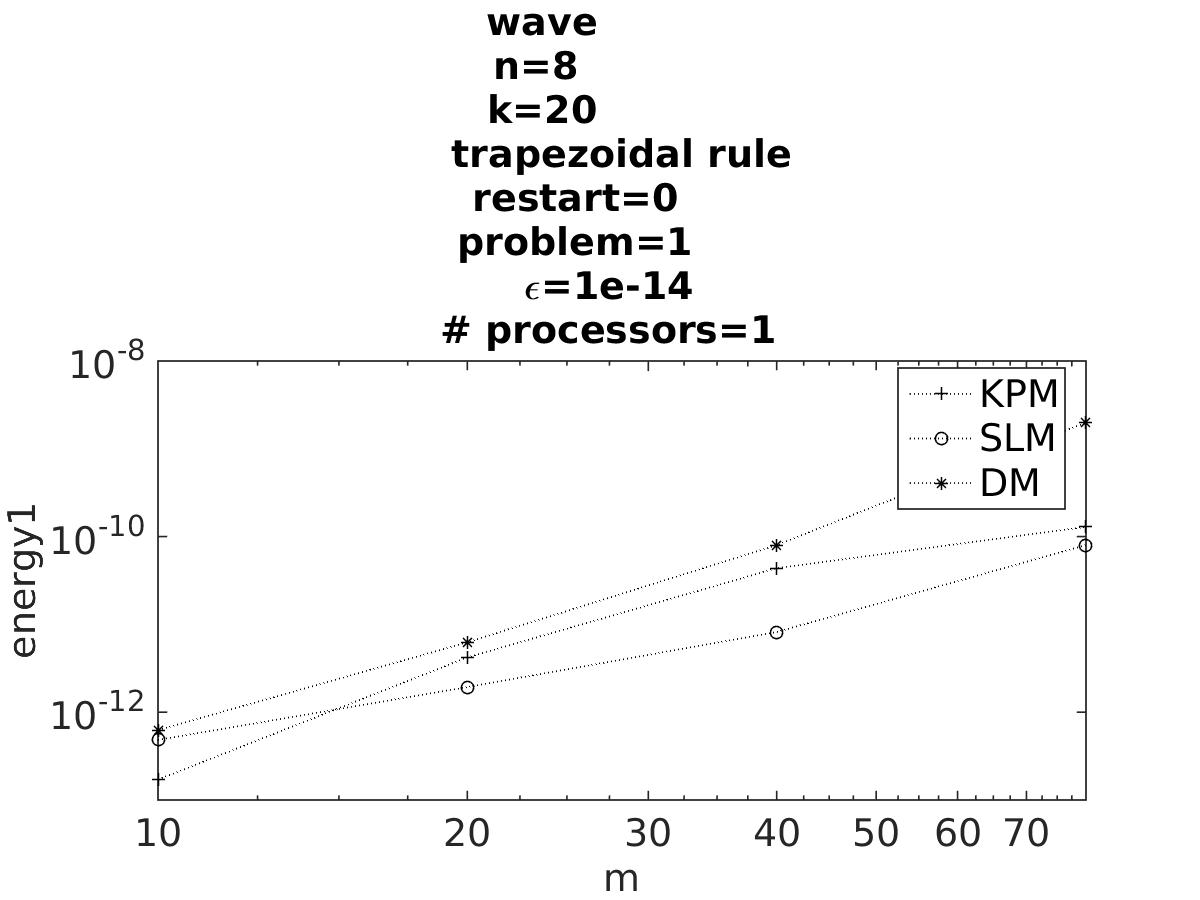
\includegraphics[width=\textwidth]{../MATLAB/fig/resultenergyr.jpg}
                \caption{  }
                \label{fig:resultenergy1}
        \end{subfigure}
        ~
        \begin{subfigure}[b]{0.45\textwidth}
                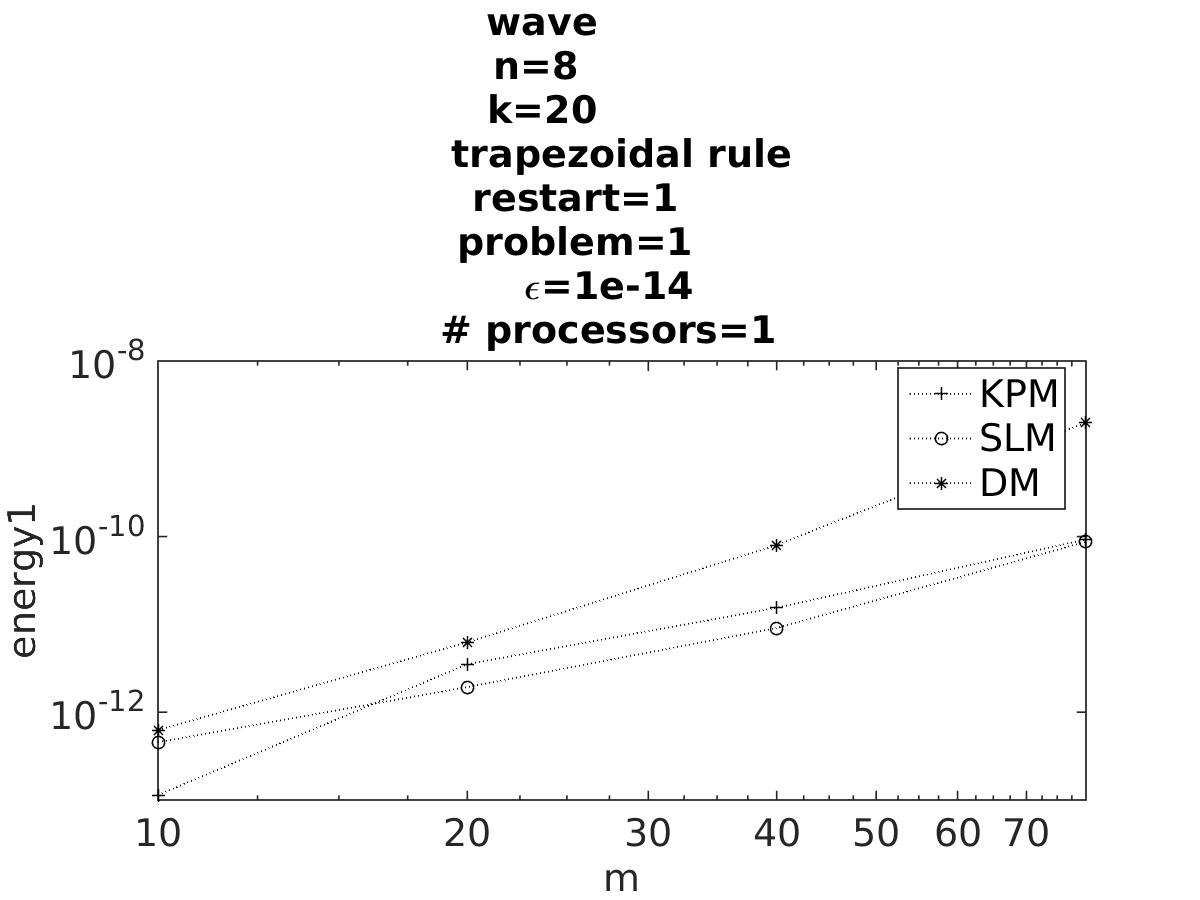
\includegraphics[width=\textwidth]{../MATLAB/fig/resultenergy.jpg}
                \caption{  }
                \label{fig:resultenergy2}
        \end{subfigure}
        \caption{ SLM and KPM has the best energy estimation, with DM not far behind. }
        \label{fig:resultenergy}
\end{figure}

It is pretty clear that the figure in this section gives no useful information about the difference between the two methods in other tings than computation time.



\section{Constant energy with the semirandom equation}
%%%%%%%%%%%%%%%%%%%%%%%%%%%%%%%%%%%%%%%%%%%%%%%%%%%%%%%%%%%%%%%%%%%%%%%%%%%%%%%%%%%%%%%%%%%%%%%%%%%%%%%



\begin{figure}[H]
        \centering
        \begin{subfigure}[b]{0.45\textwidth}
                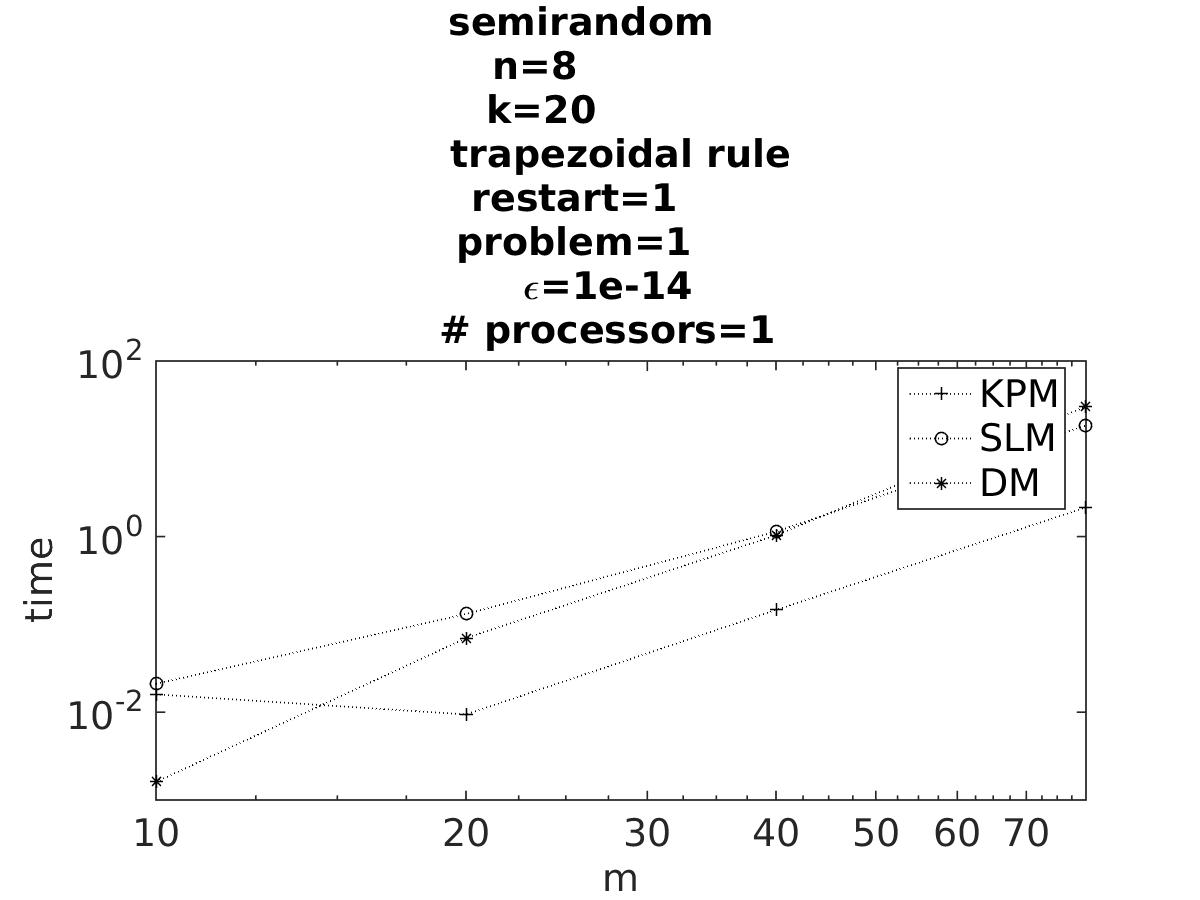
\includegraphics[width=\textwidth]{../MATLAB/fig/sresulttimem.jpg}
                \caption{  }
                \label{fig:sresulttimem}
        \end{subfigure}
        ~
        \begin{subfigure}[b]{0.45\textwidth}
                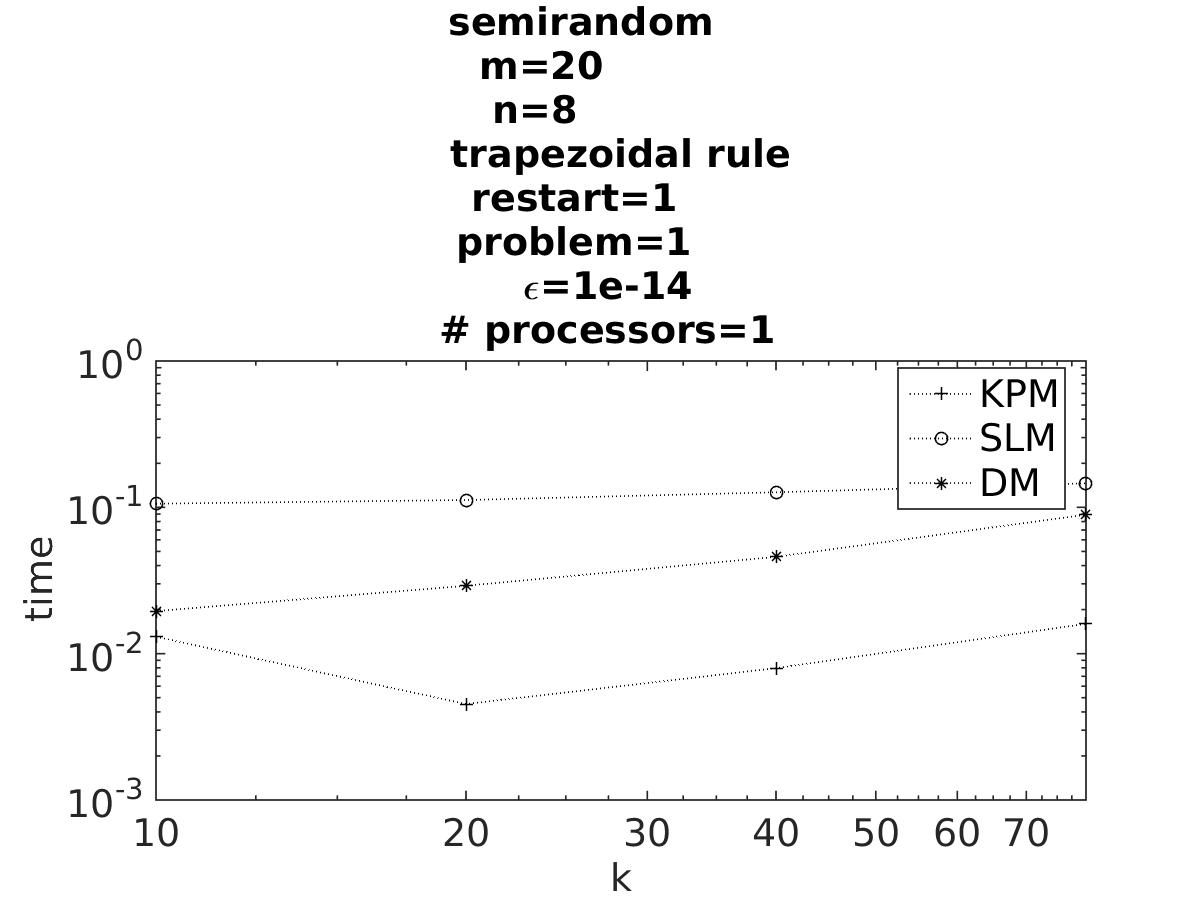
\includegraphics[width=\textwidth]{../MATLAB/fig/sresulttimek.jpg}
                \caption{  }
                \label{fig:sresulttimek}
        \end{subfigure}
        \caption{ For both cases KPM is faster than the other, and with DM faster than SLM.  }
        \label{fig:sresulttime}
\end{figure}



\begin{figure}[H]
        \centering

                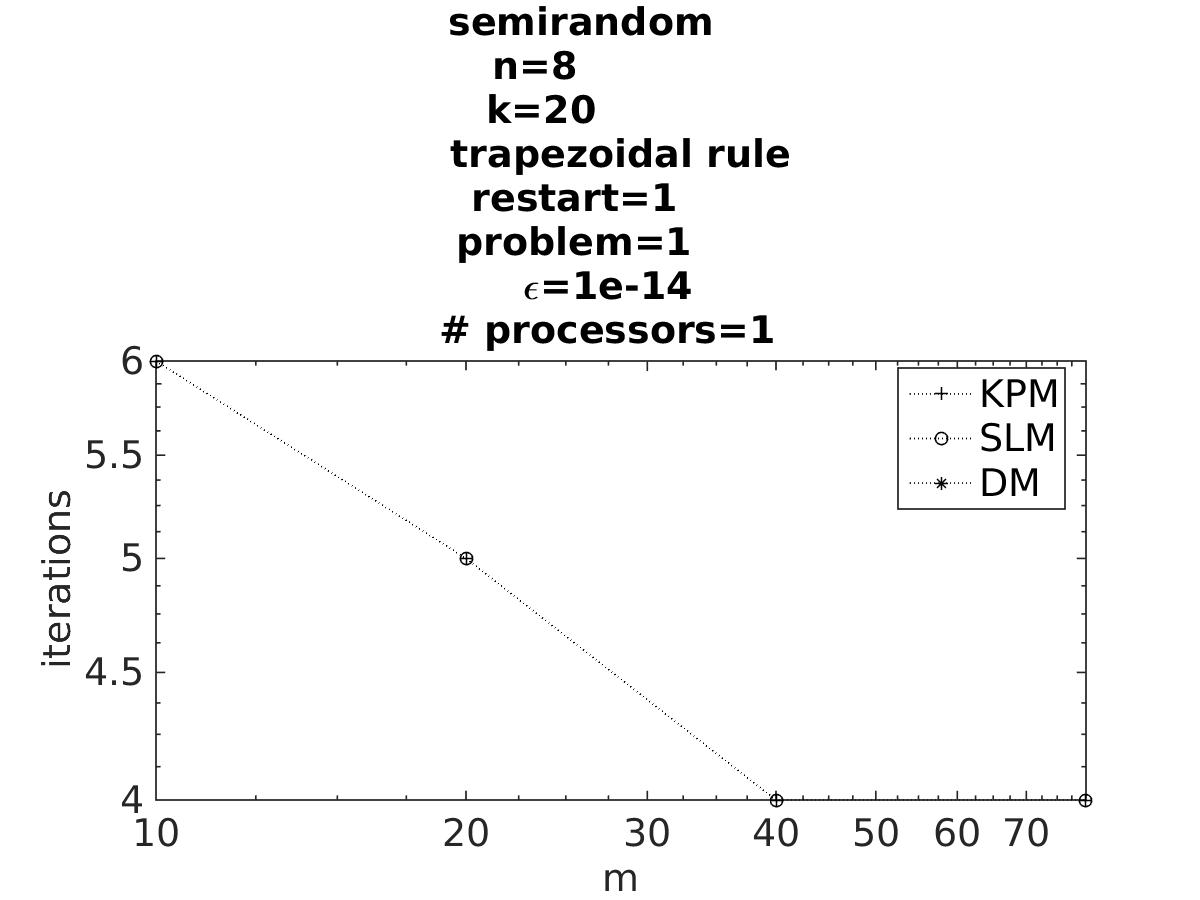
\includegraphics[width=0.45\textwidth]{../MATLAB/fig/sresultiter.jpg}
        \label{fig:sresultiter}
        \caption{The number of iterations are almost equal for the two methods.}
\end{figure}

\begin{figure}[H]
        \centering
        \begin{subfigure}[b]{0.45\textwidth}
                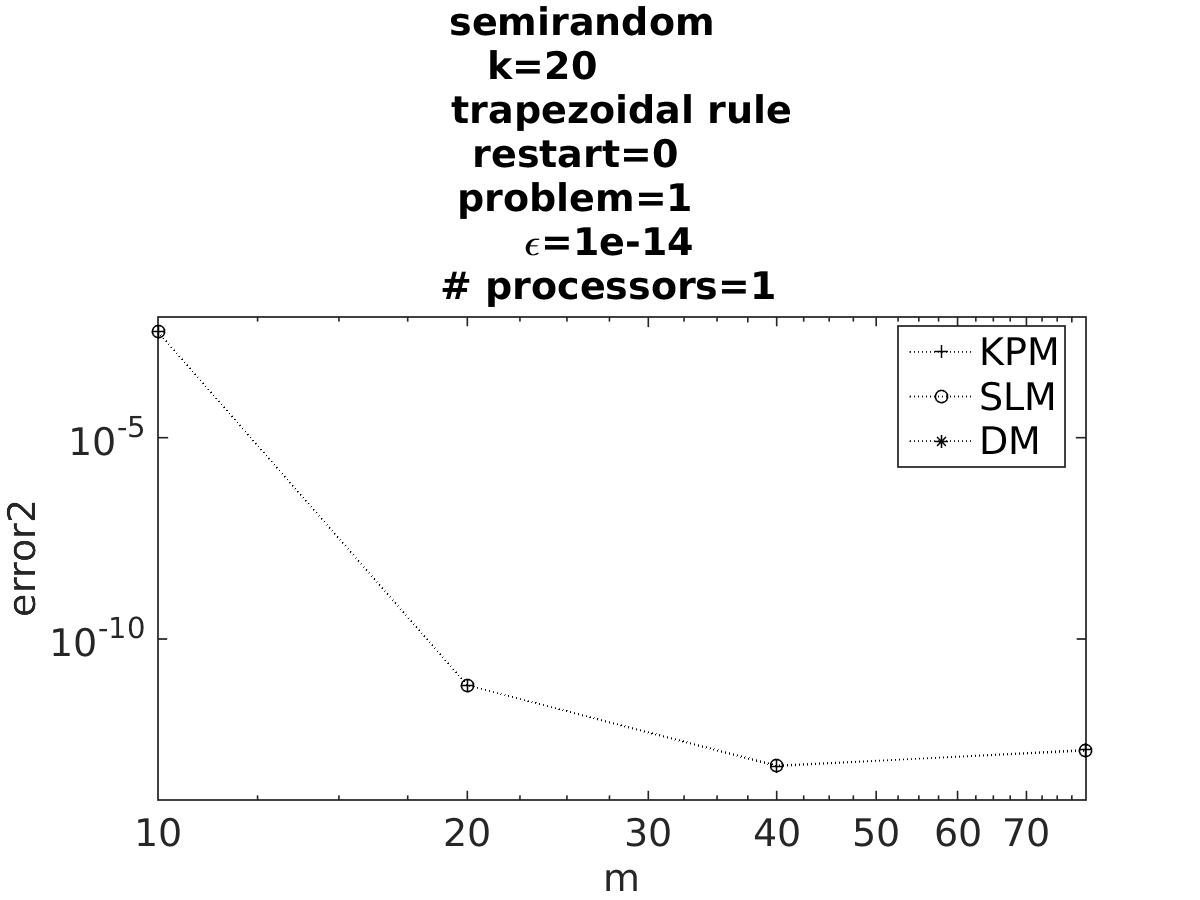
\includegraphics[width=\textwidth]{../MATLAB/fig/sresulterrorr.jpg}
                \caption{  }
                \label{fig:sresulterror1}
        \end{subfigure}
        ~
        \begin{subfigure}[b]{0.45\textwidth}
                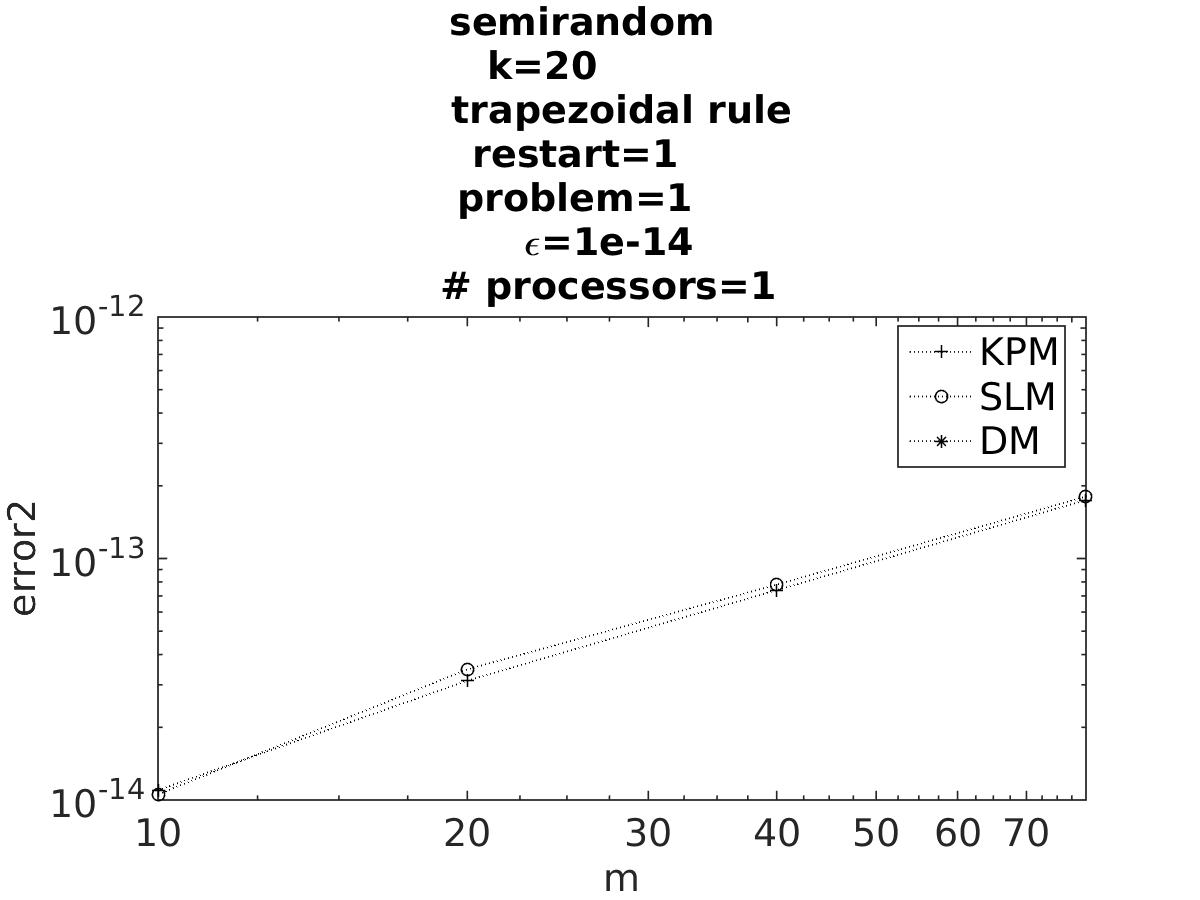
\includegraphics[width=\textwidth]{../MATLAB/fig/sresulterror.jpg}
                \caption{  }
                \label{fig:sresulterror2}
        \end{subfigure}
        \caption{ The error is nearly identical.  }
        \label{fig:sresulterror}
\end{figure}


\begin{figure}[H]
        \centering
        \begin{subfigure}[b]{0.45\textwidth}
                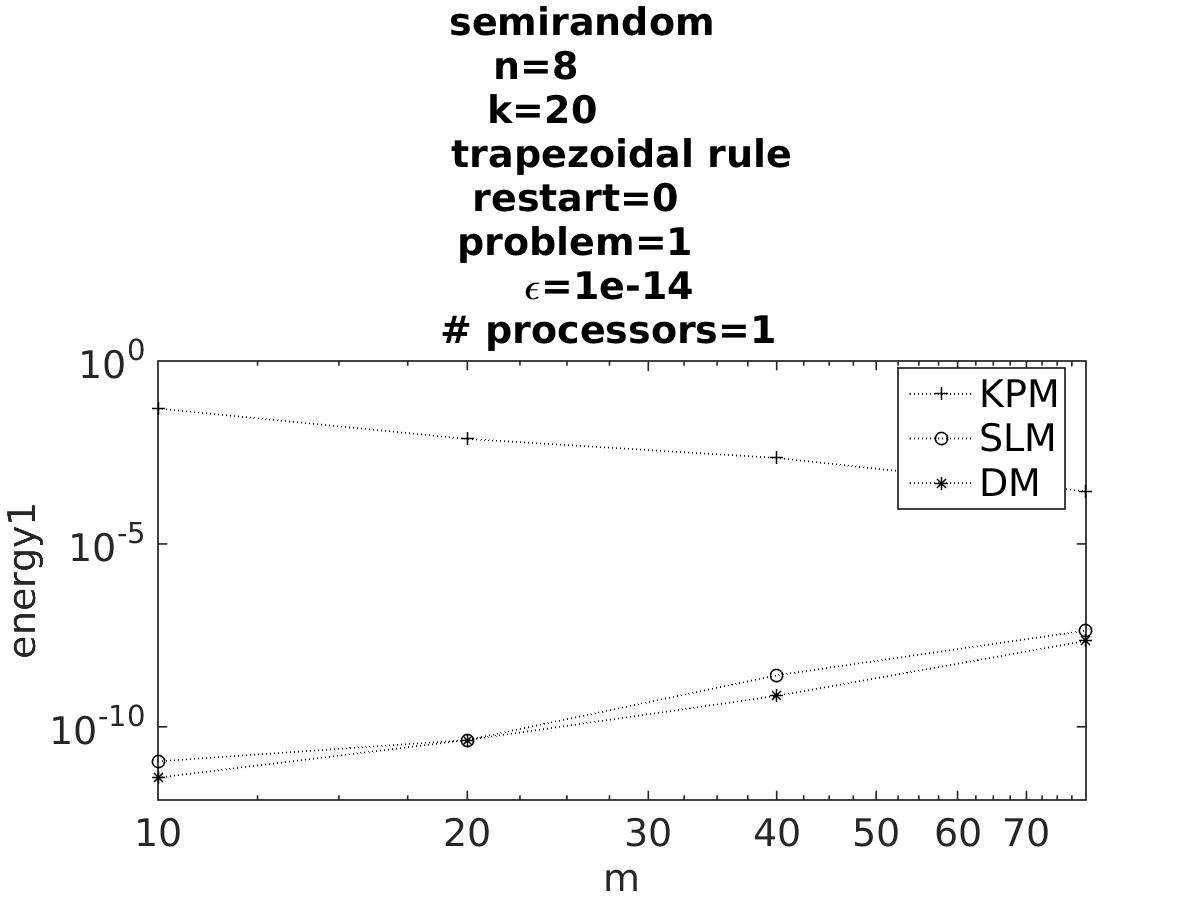
\includegraphics[width=\textwidth]{../MATLAB/fig/sresultenergyr.jpg}
                \caption{  }
                \label{fig:sresultenergy1}
        \end{subfigure}
        ~
        \begin{subfigure}[b]{0.45\textwidth}
                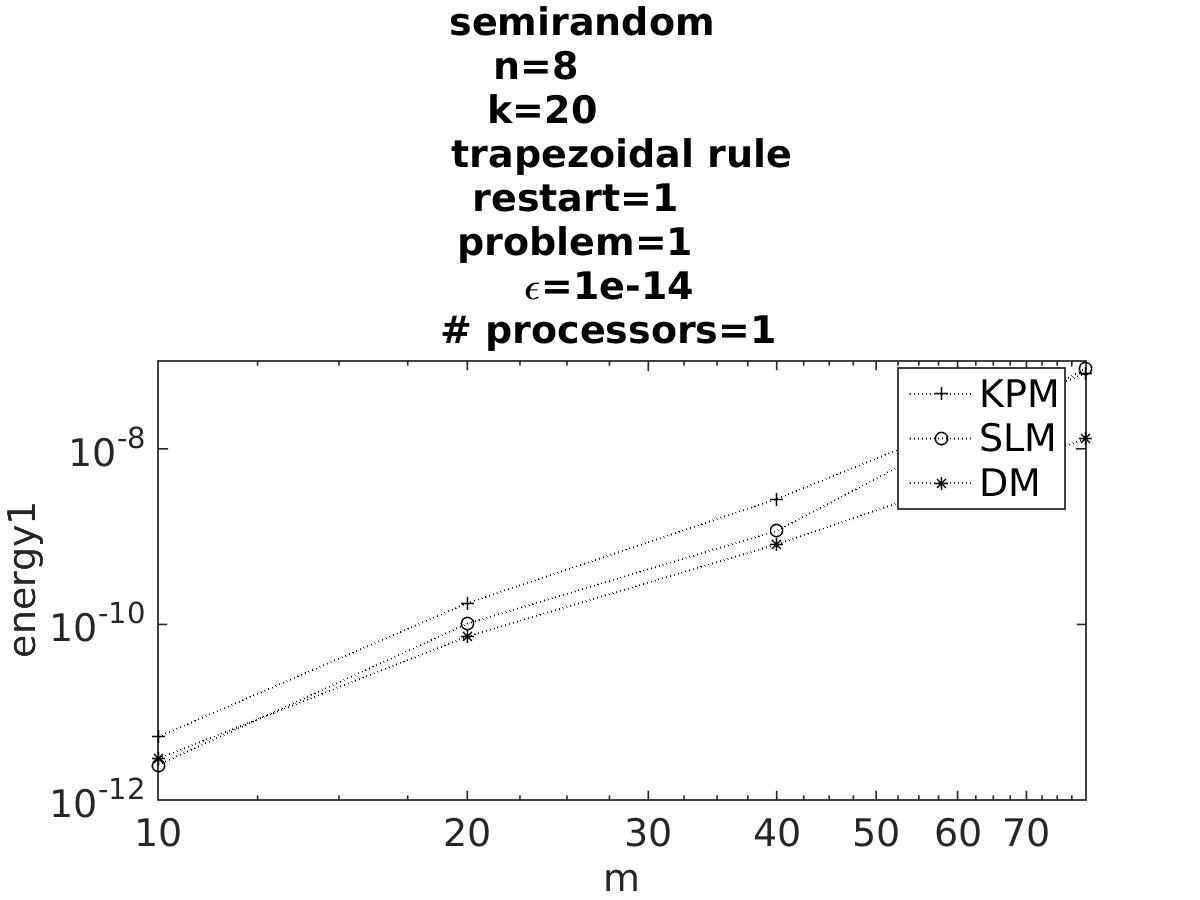
\includegraphics[width=\textwidth]{../MATLAB/fig/sresultenergy.jpg}
                \caption{  }
                \label{fig:sresultenergy2}
        \end{subfigure}
        \caption{ SLM and KPM has the best energy estimation, with DM not far behind. }
        \label{fig:sresultenergy}
\end{figure}

The figures in this section shows a little better how the energy for the different methods change, but the error is apparently useless in this setting due to it being the difference between two calculated numbers, and not the analytical solution. 

\section{Varying energy with the wave equation}
%%%%%%%%%%%%%%%%%%%%%%%%%%%%%%%%%%%%%%%%%%%%%%%%%%%%%%%%%%%%%%%%%%%%%%%%%%%%%%%%%%%%%%%%%%%%%%%%%%%%%%%
\begin{figure}[H]
        \centering
        \begin{subfigure}[b]{0.45\textwidth}
                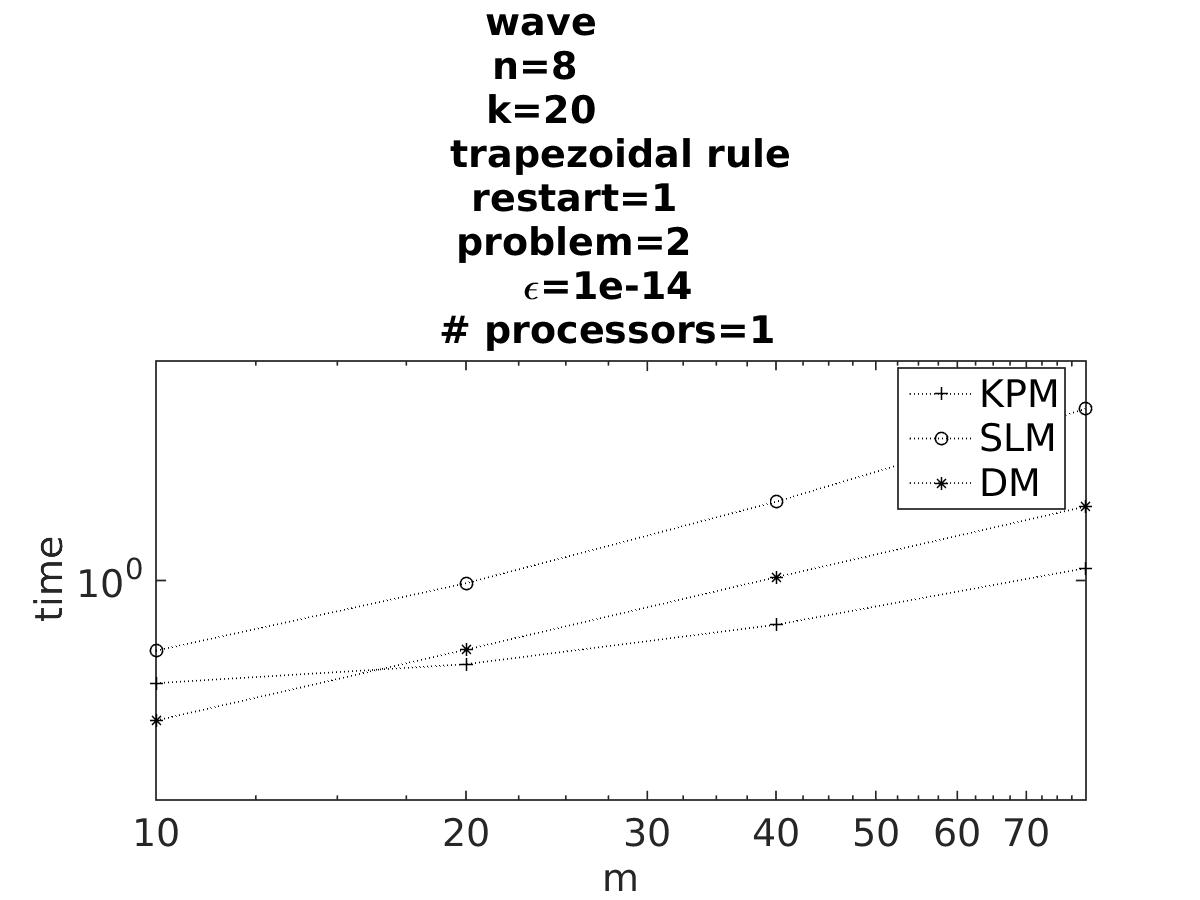
\includegraphics[width=\textwidth]{../MATLAB/fig/vresulttimem.jpg}
                \caption{  }
                \label{fig:vresulttimem}
        \end{subfigure}
        ~
        \begin{subfigure}[b]{0.45\textwidth}
                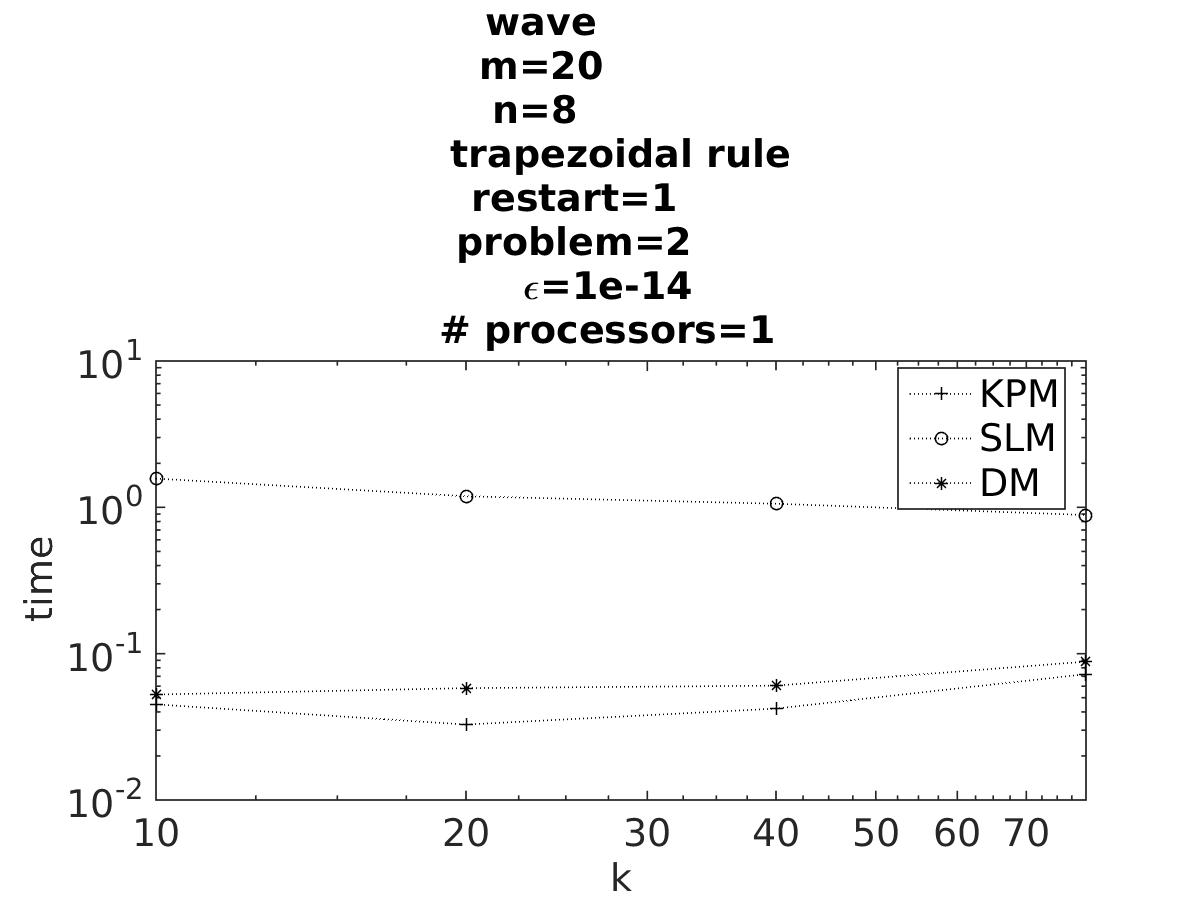
\includegraphics[width=\textwidth]{../MATLAB/fig/vresulttimek.jpg}
                \caption{  }
                \label{fig:vresulttimek}
        \end{subfigure}
        \caption{ For both cases KPM is faster than the other, and with DM faster than SLM.  }
        \label{fig:vresulttime}
\end{figure}



\begin{figure}[H]
        \centering

                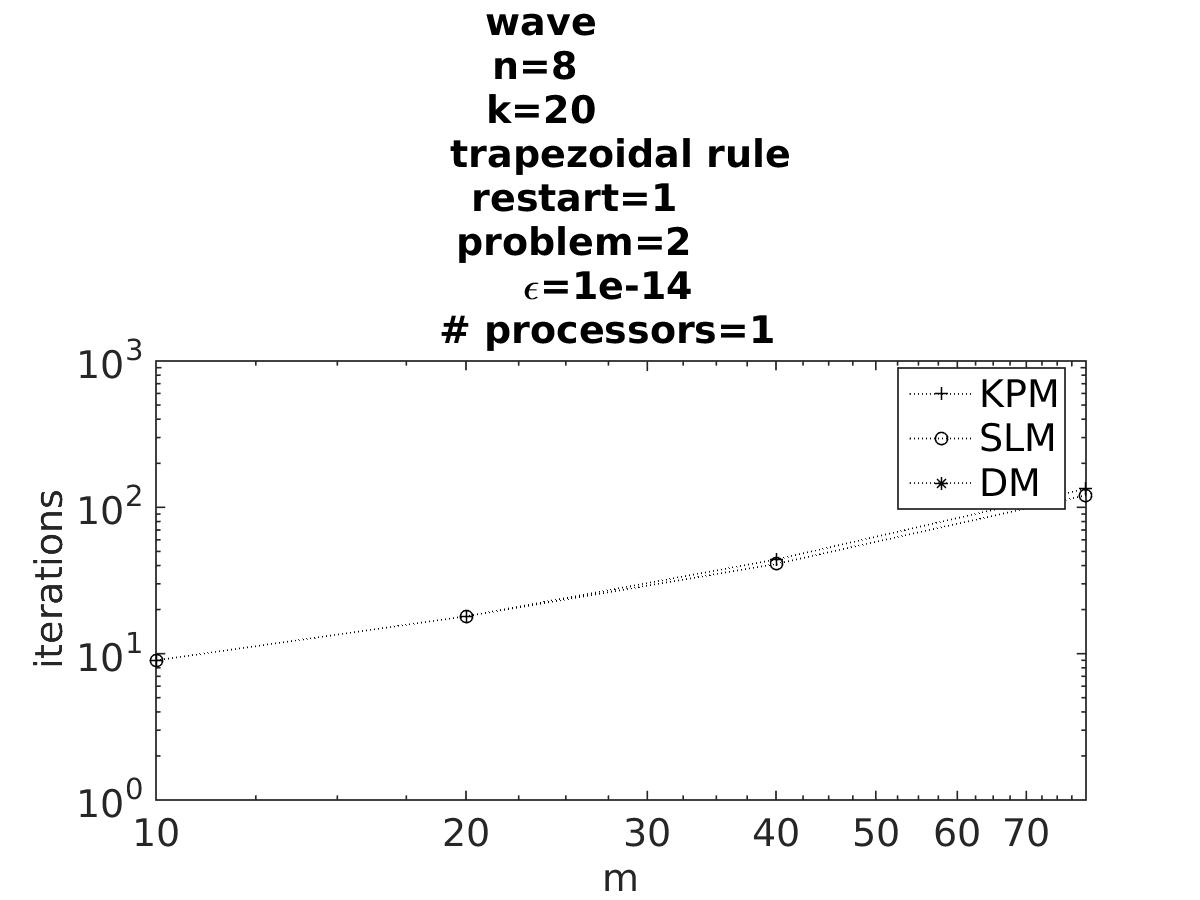
\includegraphics[width=0.45\textwidth]{../MATLAB/fig/vresultiter.jpg}
        \label{fig:vresultiter}
        \caption{The number of iterations are almost equal for the two methods.}
\end{figure}

\begin{figure}[H]
        \centering
        \begin{subfigure}[b]{0.45\textwidth}
                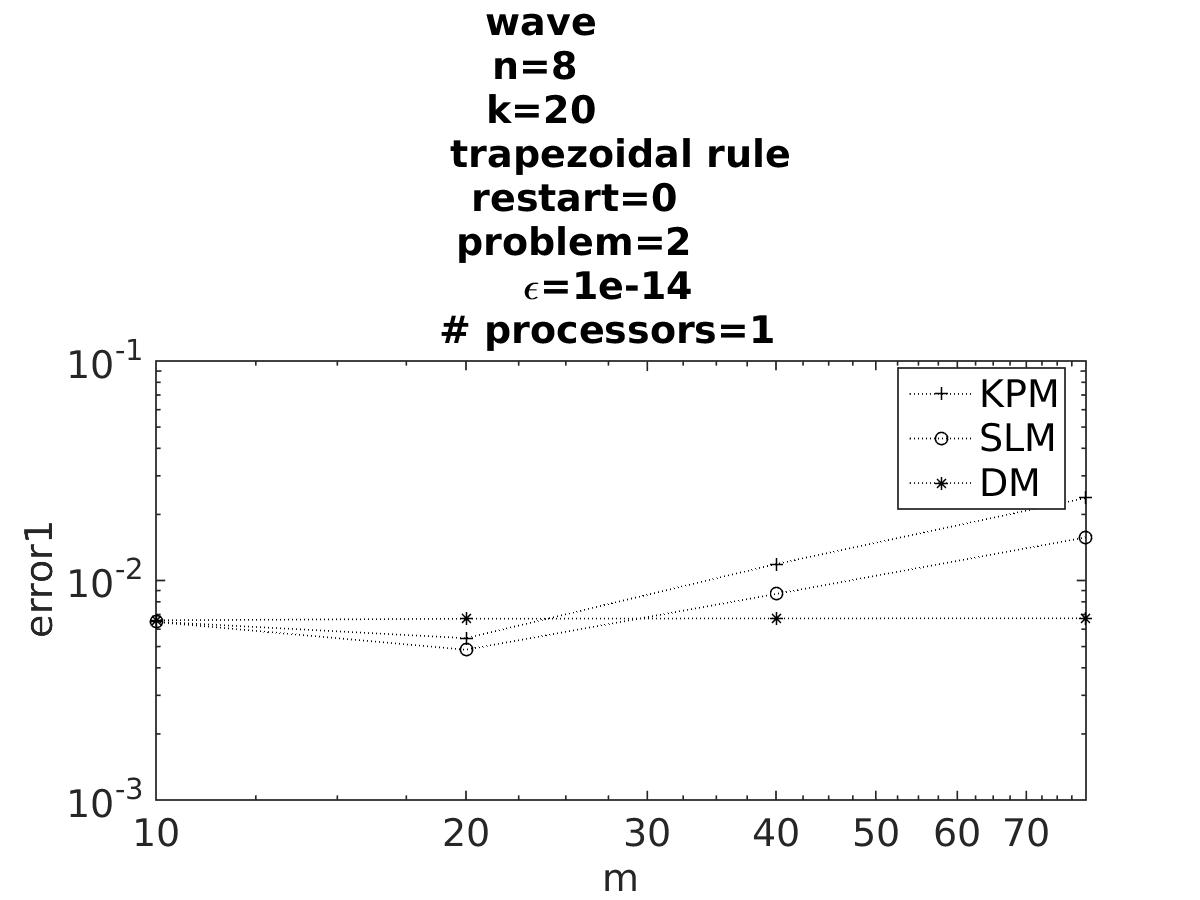
\includegraphics[width=\textwidth]{../MATLAB/fig/vresulterrorr.jpg}
                \caption{  }
                \label{fig:vresulterror1}
        \end{subfigure}
        ~
        \begin{subfigure}[b]{0.45\textwidth}
                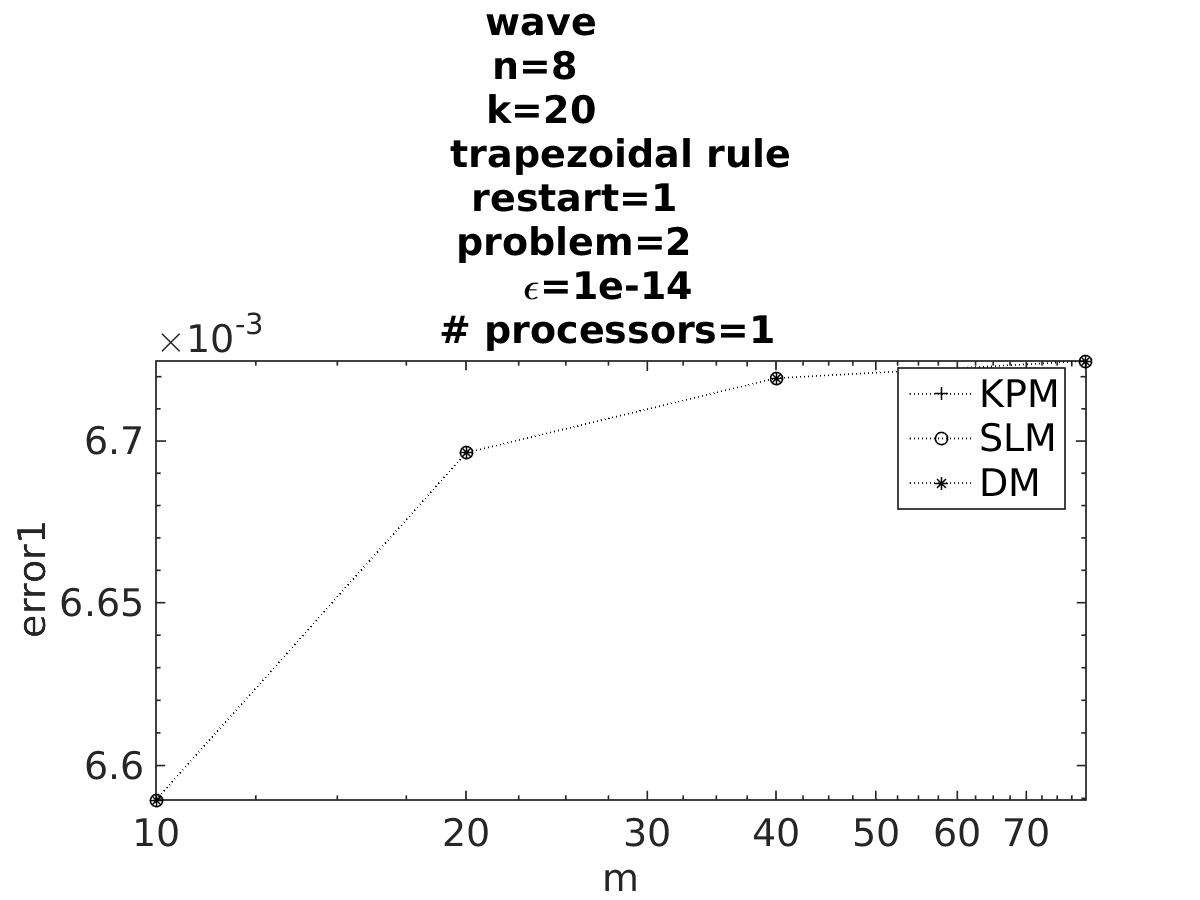
\includegraphics[width=\textwidth]{../MATLAB/fig/vresulterror.jpg}
                \caption{  }
                \label{fig:vresulterror2}
        \end{subfigure}
        \caption{ The error is nearly identical.  }
        \label{fig:vresulterror}
\end{figure}


\begin{figure}[H]
        \centering
        \begin{subfigure}[b]{0.45\textwidth}
                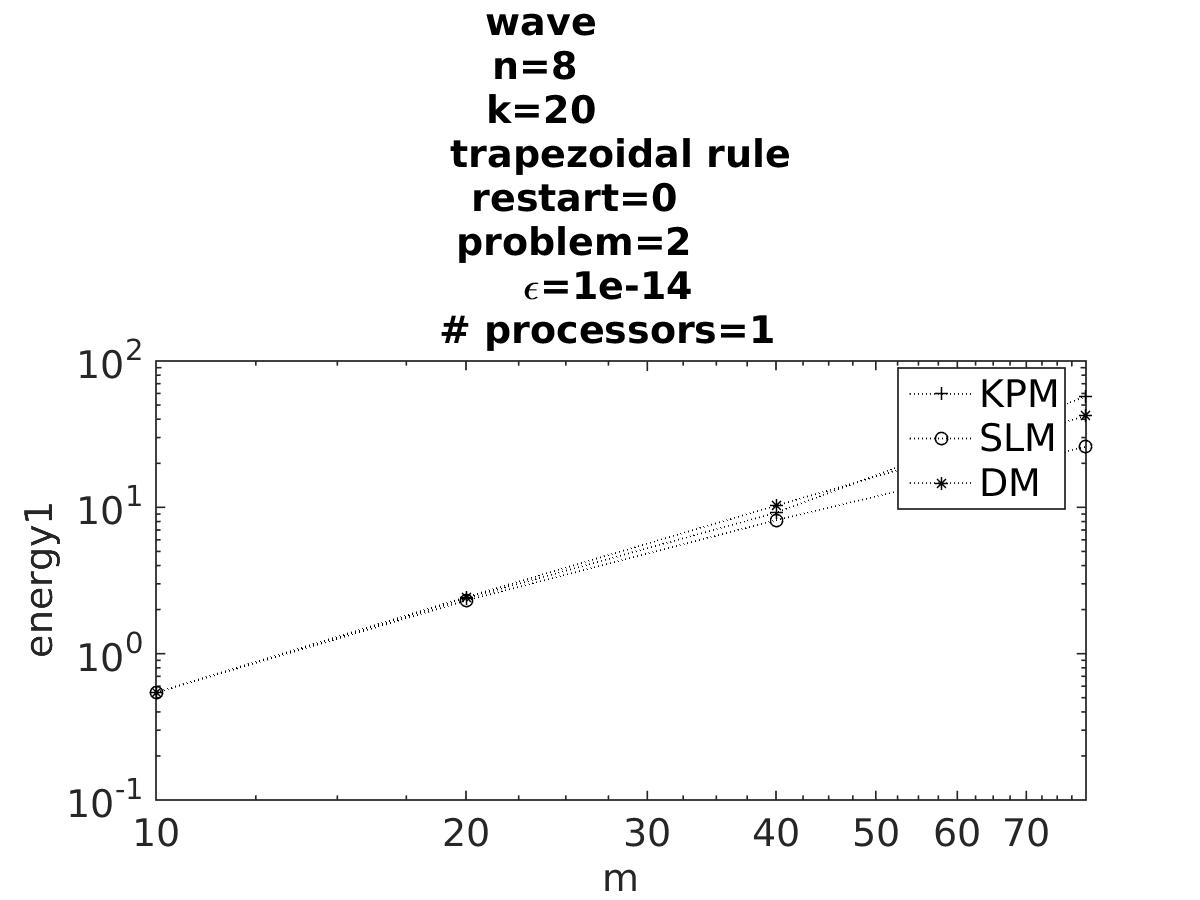
\includegraphics[width=\textwidth]{../MATLAB/fig/vresultenergyr.jpg}
                \caption{  }
                \label{fig:vresultenergy1}
        \end{subfigure}
        ~
        \begin{subfigure}[b]{0.45\textwidth}
                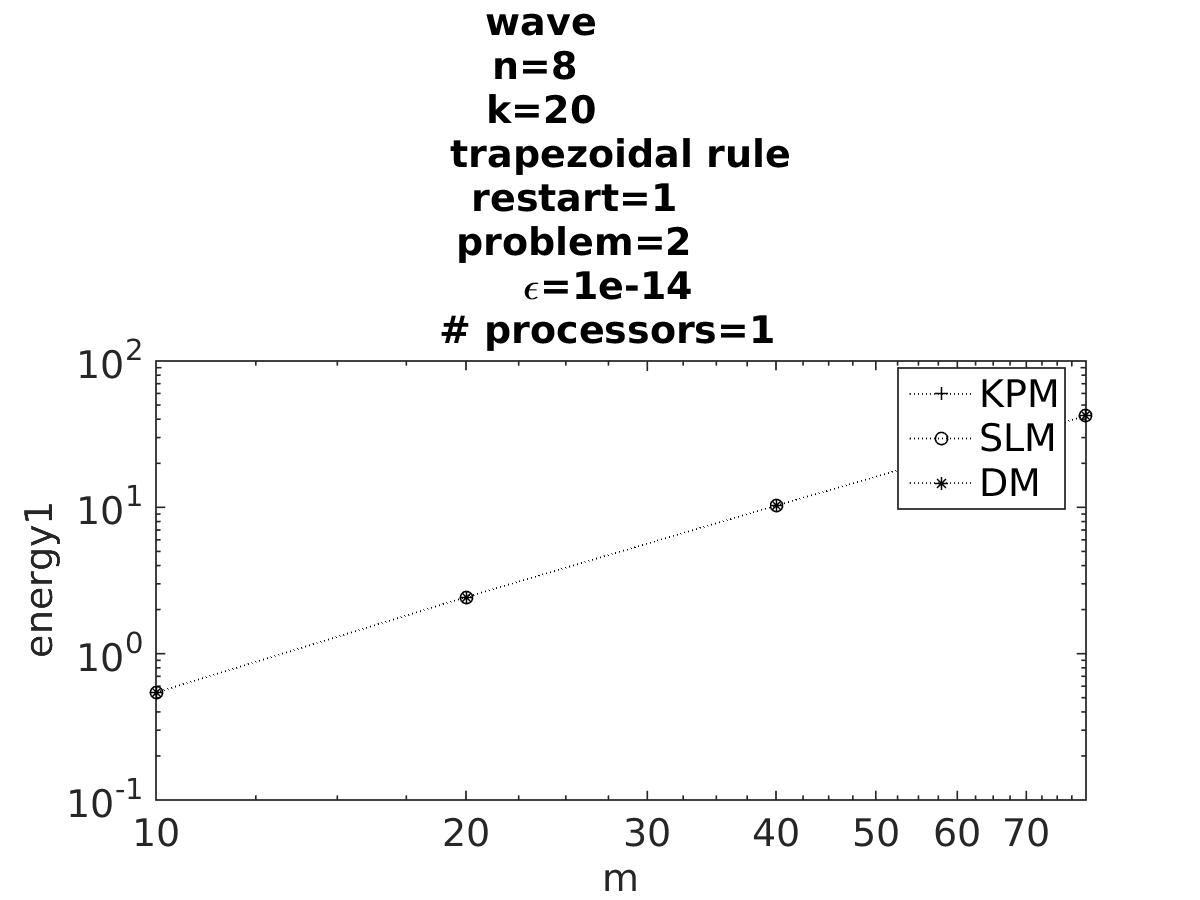
\includegraphics[width=\textwidth]{../MATLAB/fig/vresultenergy.jpg}
                \caption{  }
                \label{fig:vresultenergy2}
        \end{subfigure}
        \caption{ SLM and KPM has the best energy estimation, with DM not far behind. }
        \label{fig:vresultenergy}
\end{figure}

\section{Varying energy with the semirandom equation}
%%%%%%%%%%%%%%%%%%%%%%%%%%%%%%%%%%%%%%%%%%%%%%%%%%%%%%%%%%%%%%%%%%%%%%%%%%%%%%%%%%%%%%%%%%%%%%%%%%%%%%%

\begin{figure}[H]
        \centering
        \begin{subfigure}[b]{0.45\textwidth}
                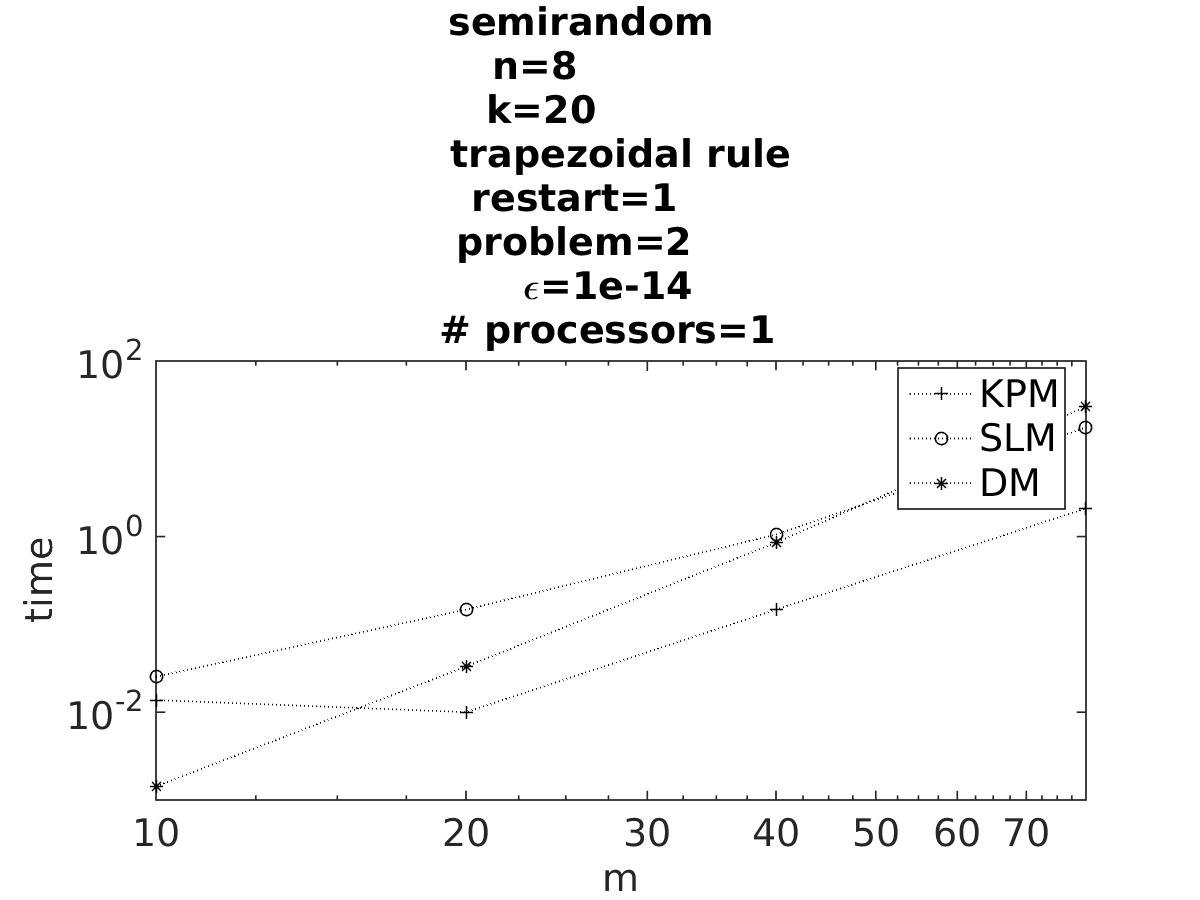
\includegraphics[width=\textwidth]{../MATLAB/fig/vsresulttimem.jpg}
                \caption{  }
                \label{fig:vsresulttimem}
        \end{subfigure}
        ~
        \begin{subfigure}[b]{0.45\textwidth}
                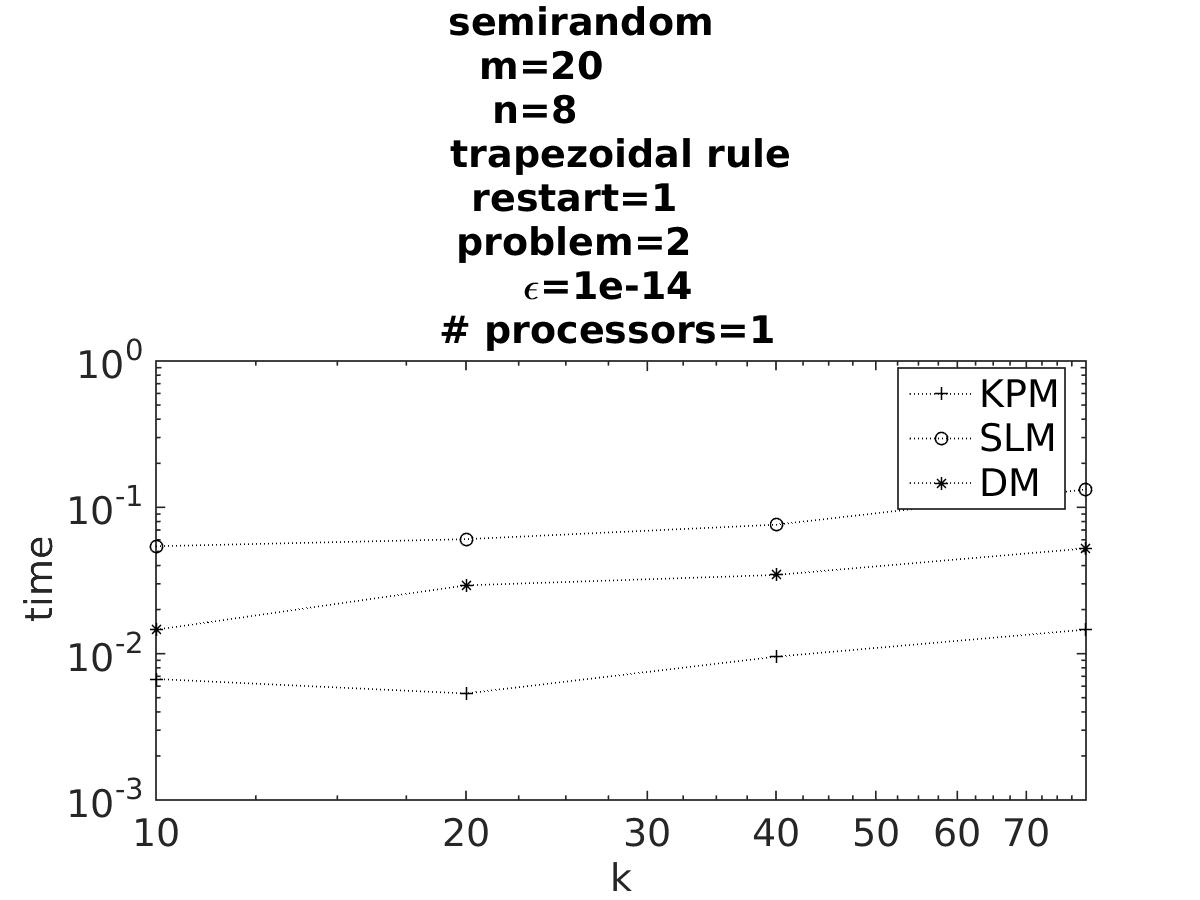
\includegraphics[width=\textwidth]{../MATLAB/fig/vsresulttimek.jpg}
                \caption{  }
                \label{fig:vsresulttimek}
        \end{subfigure}
        \caption{ For both cases KPM is faster than the other, and with DM faster than SLM.  }
        \label{fig:vsresulttime}
\end{figure}



\begin{figure}[H]
        \centering

                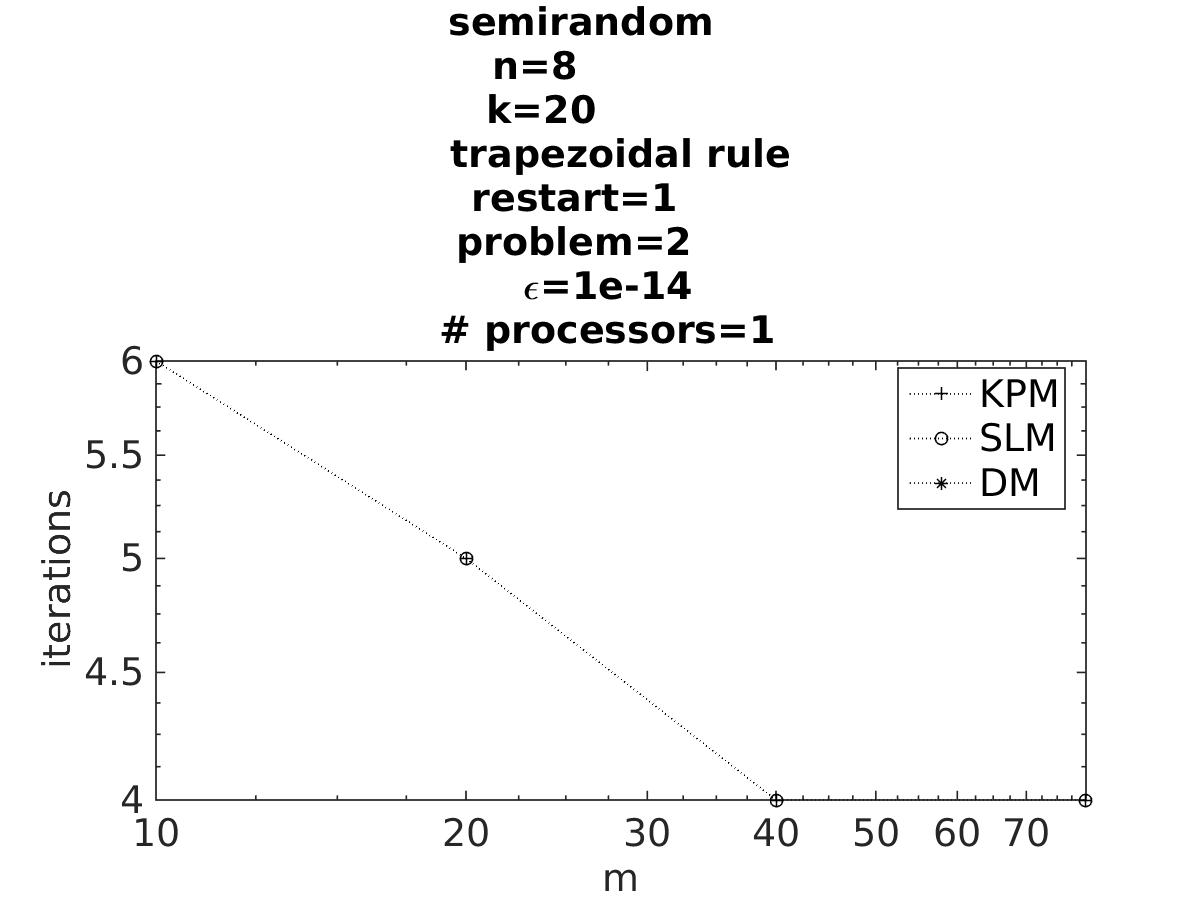
\includegraphics[width=0.45\textwidth]{../MATLAB/fig/vsresultiter.jpg}
        \label{fig:vsresultiter}
        \caption{The number of iterations are almost equal for the two methods.}
\end{figure}

\begin{figure}[H]
        \centering
        \begin{subfigure}[b]{0.45\textwidth}
                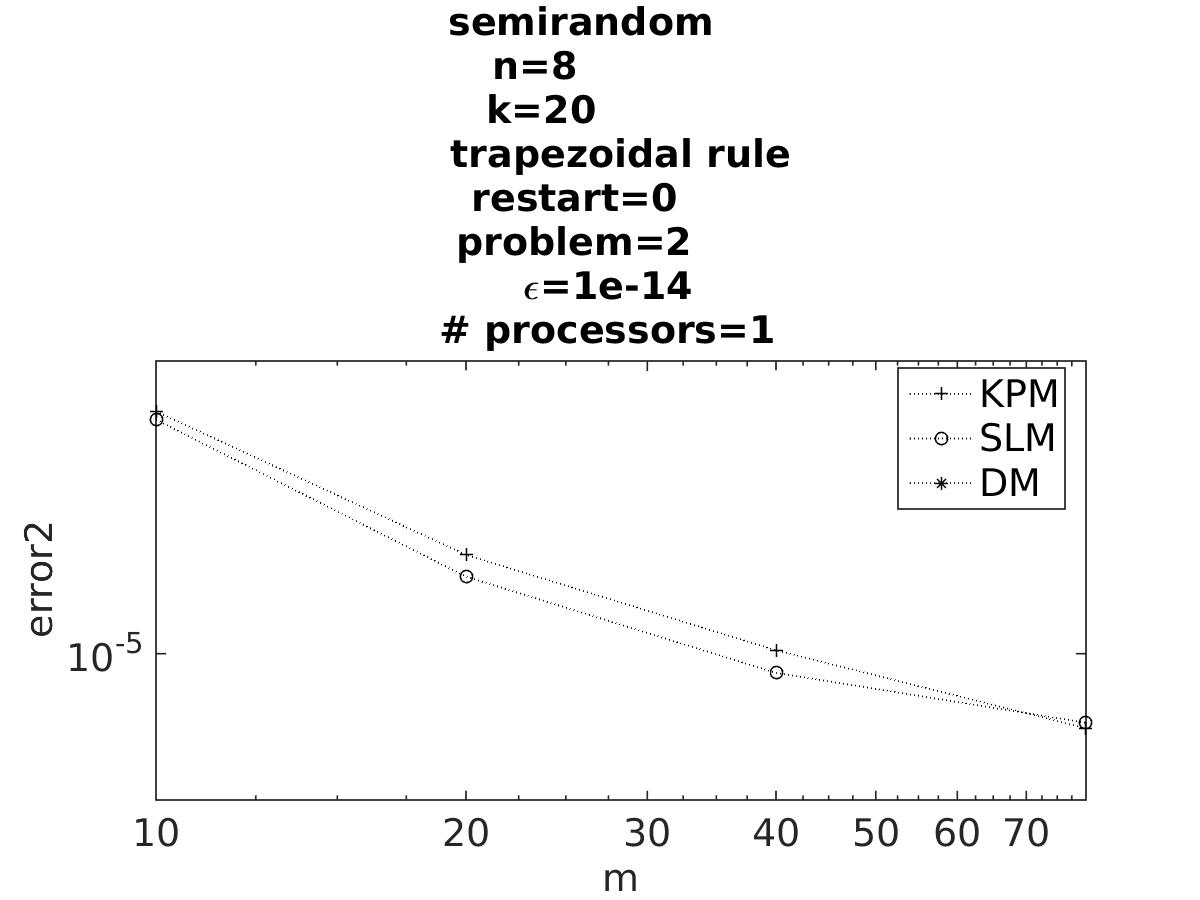
\includegraphics[width=\textwidth]{../MATLAB/fig/vsresulterrorr.jpg}
                \caption{  }
                \label{fig:vsresulterror1}
        \end{subfigure}
        ~
        \begin{subfigure}[b]{0.45\textwidth}
                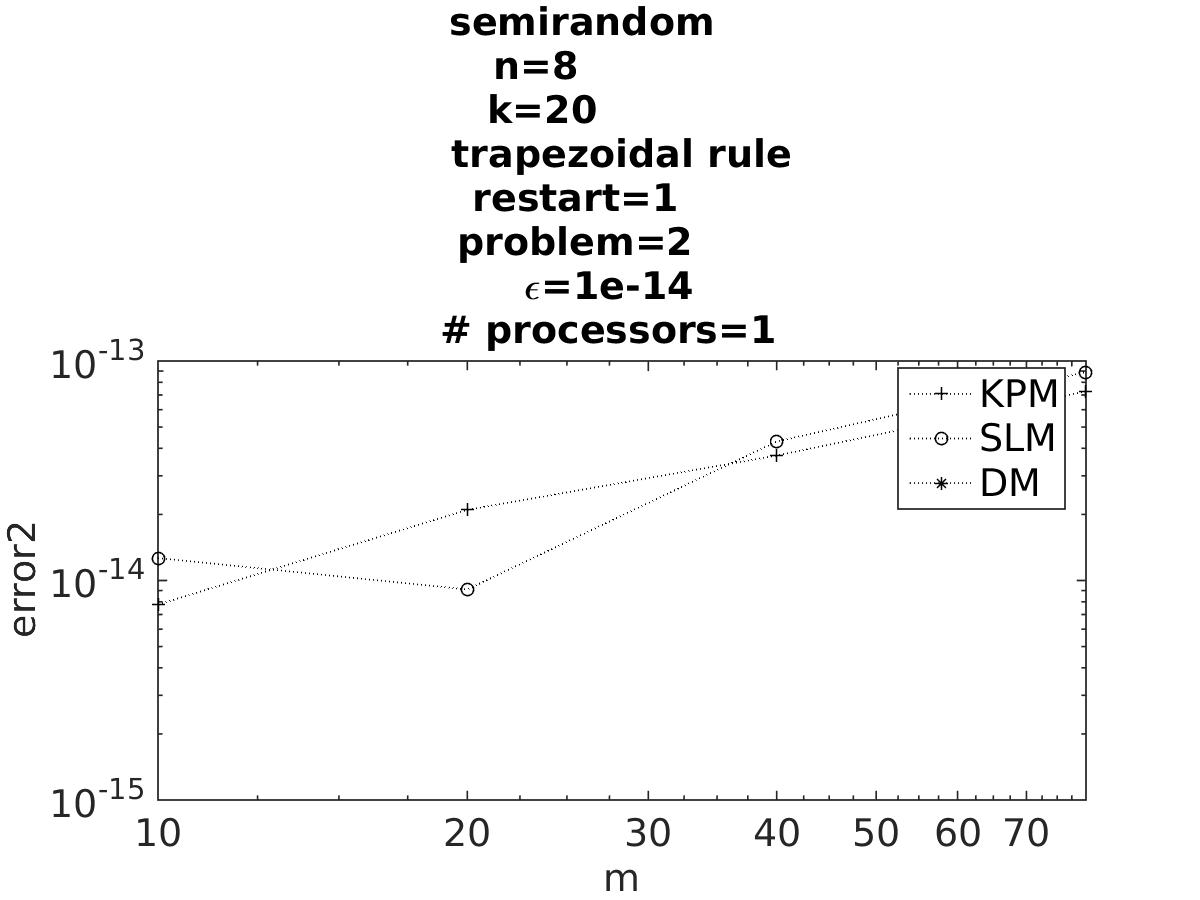
\includegraphics[width=\textwidth]{../MATLAB/fig/vsresulterror.jpg}
                \caption{  }
                \label{fig:vsresulterror2}
        \end{subfigure}
        \caption{ The error is nearly identical.  }
        \label{fig:vsresulterror}
\end{figure}


\begin{figure}[H]
        \centering
        \begin{subfigure}[b]{0.45\textwidth}
                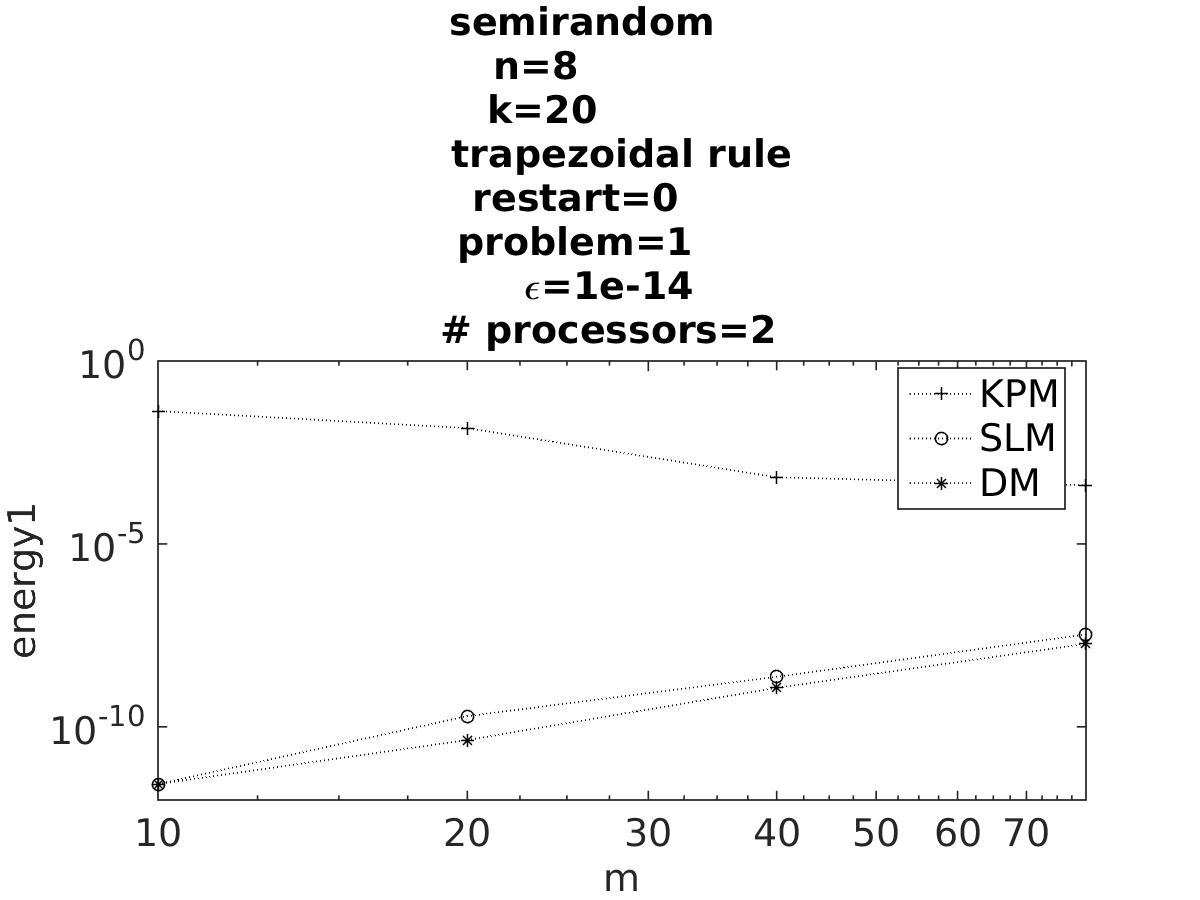
\includegraphics[width=\textwidth]{../MATLAB/fig/vsresultenergyr.jpg}
                \caption{  }
                \label{fig:vsresultenergy1}
        \end{subfigure}
        ~
        \begin{subfigure}[b]{0.45\textwidth}
                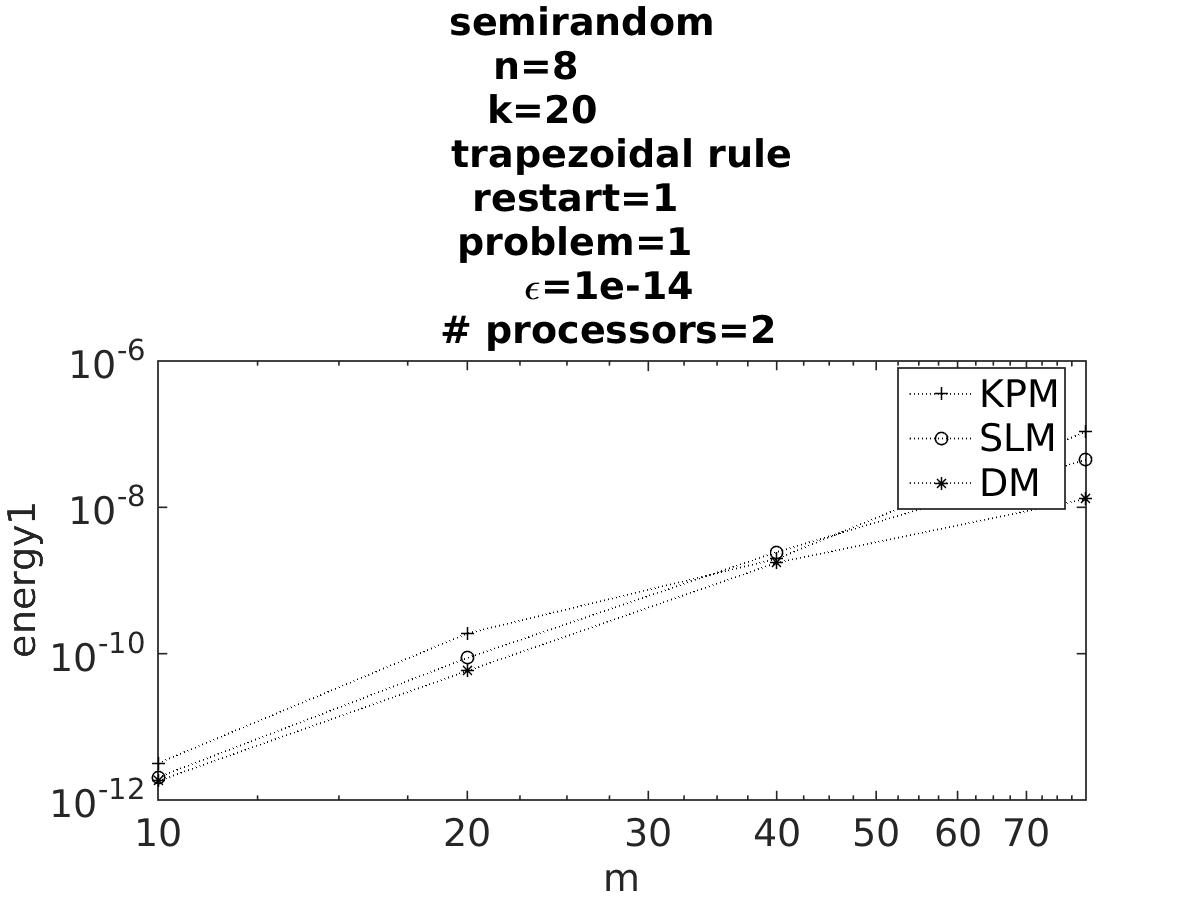
\includegraphics[width=\textwidth]{../MATLAB/fig/vsresultenergy.jpg}
                \caption{  }
                \label{fig:vsresultenergy2}
        \end{subfigure}
        \caption{ SLM and KPM has the best energy estimation, with DM not far behind. }
        \label{fig:vsresultenergy}
\end{figure}
It is clear that the restart improves the energy estimates for 